% Options for packages loaded elsewhere
\PassOptionsToPackage{unicode}{hyperref}
\PassOptionsToPackage{hyphens}{url}
%
\documentclass[
]{book}
\usepackage{amsmath,amssymb}
\usepackage{iftex}
\ifPDFTeX
  \usepackage[T1]{fontenc}
  \usepackage[utf8]{inputenc}
  \usepackage{textcomp} % provide euro and other symbols
\else % if luatex or xetex
  \usepackage{unicode-math} % this also loads fontspec
  \defaultfontfeatures{Scale=MatchLowercase}
  \defaultfontfeatures[\rmfamily]{Ligatures=TeX,Scale=1}
\fi
\usepackage{lmodern}
\ifPDFTeX\else
  % xetex/luatex font selection
\fi
% Use upquote if available, for straight quotes in verbatim environments
\IfFileExists{upquote.sty}{\usepackage{upquote}}{}
\IfFileExists{microtype.sty}{% use microtype if available
  \usepackage[]{microtype}
  \UseMicrotypeSet[protrusion]{basicmath} % disable protrusion for tt fonts
}{}
\makeatletter
\@ifundefined{KOMAClassName}{% if non-KOMA class
  \IfFileExists{parskip.sty}{%
    \usepackage{parskip}
  }{% else
    \setlength{\parindent}{0pt}
    \setlength{\parskip}{6pt plus 2pt minus 1pt}}
}{% if KOMA class
  \KOMAoptions{parskip=half}}
\makeatother
\usepackage{xcolor}
\usepackage{color}
\usepackage{fancyvrb}
\newcommand{\VerbBar}{|}
\newcommand{\VERB}{\Verb[commandchars=\\\{\}]}
\DefineVerbatimEnvironment{Highlighting}{Verbatim}{commandchars=\\\{\}}
% Add ',fontsize=\small' for more characters per line
\usepackage{framed}
\definecolor{shadecolor}{RGB}{248,248,248}
\newenvironment{Shaded}{\begin{snugshade}}{\end{snugshade}}
\newcommand{\AlertTok}[1]{\textcolor[rgb]{0.94,0.16,0.16}{#1}}
\newcommand{\AnnotationTok}[1]{\textcolor[rgb]{0.56,0.35,0.01}{\textbf{\textit{#1}}}}
\newcommand{\AttributeTok}[1]{\textcolor[rgb]{0.13,0.29,0.53}{#1}}
\newcommand{\BaseNTok}[1]{\textcolor[rgb]{0.00,0.00,0.81}{#1}}
\newcommand{\BuiltInTok}[1]{#1}
\newcommand{\CharTok}[1]{\textcolor[rgb]{0.31,0.60,0.02}{#1}}
\newcommand{\CommentTok}[1]{\textcolor[rgb]{0.56,0.35,0.01}{\textit{#1}}}
\newcommand{\CommentVarTok}[1]{\textcolor[rgb]{0.56,0.35,0.01}{\textbf{\textit{#1}}}}
\newcommand{\ConstantTok}[1]{\textcolor[rgb]{0.56,0.35,0.01}{#1}}
\newcommand{\ControlFlowTok}[1]{\textcolor[rgb]{0.13,0.29,0.53}{\textbf{#1}}}
\newcommand{\DataTypeTok}[1]{\textcolor[rgb]{0.13,0.29,0.53}{#1}}
\newcommand{\DecValTok}[1]{\textcolor[rgb]{0.00,0.00,0.81}{#1}}
\newcommand{\DocumentationTok}[1]{\textcolor[rgb]{0.56,0.35,0.01}{\textbf{\textit{#1}}}}
\newcommand{\ErrorTok}[1]{\textcolor[rgb]{0.64,0.00,0.00}{\textbf{#1}}}
\newcommand{\ExtensionTok}[1]{#1}
\newcommand{\FloatTok}[1]{\textcolor[rgb]{0.00,0.00,0.81}{#1}}
\newcommand{\FunctionTok}[1]{\textcolor[rgb]{0.13,0.29,0.53}{\textbf{#1}}}
\newcommand{\ImportTok}[1]{#1}
\newcommand{\InformationTok}[1]{\textcolor[rgb]{0.56,0.35,0.01}{\textbf{\textit{#1}}}}
\newcommand{\KeywordTok}[1]{\textcolor[rgb]{0.13,0.29,0.53}{\textbf{#1}}}
\newcommand{\NormalTok}[1]{#1}
\newcommand{\OperatorTok}[1]{\textcolor[rgb]{0.81,0.36,0.00}{\textbf{#1}}}
\newcommand{\OtherTok}[1]{\textcolor[rgb]{0.56,0.35,0.01}{#1}}
\newcommand{\PreprocessorTok}[1]{\textcolor[rgb]{0.56,0.35,0.01}{\textit{#1}}}
\newcommand{\RegionMarkerTok}[1]{#1}
\newcommand{\SpecialCharTok}[1]{\textcolor[rgb]{0.81,0.36,0.00}{\textbf{#1}}}
\newcommand{\SpecialStringTok}[1]{\textcolor[rgb]{0.31,0.60,0.02}{#1}}
\newcommand{\StringTok}[1]{\textcolor[rgb]{0.31,0.60,0.02}{#1}}
\newcommand{\VariableTok}[1]{\textcolor[rgb]{0.00,0.00,0.00}{#1}}
\newcommand{\VerbatimStringTok}[1]{\textcolor[rgb]{0.31,0.60,0.02}{#1}}
\newcommand{\WarningTok}[1]{\textcolor[rgb]{0.56,0.35,0.01}{\textbf{\textit{#1}}}}
\usepackage{longtable,booktabs,array}
\usepackage{calc} % for calculating minipage widths
% Correct order of tables after \paragraph or \subparagraph
\usepackage{etoolbox}
\makeatletter
\patchcmd\longtable{\par}{\if@noskipsec\mbox{}\fi\par}{}{}
\makeatother
% Allow footnotes in longtable head/foot
\IfFileExists{footnotehyper.sty}{\usepackage{footnotehyper}}{\usepackage{footnote}}
\makesavenoteenv{longtable}
\usepackage{graphicx}
\makeatletter
\def\maxwidth{\ifdim\Gin@nat@width>\linewidth\linewidth\else\Gin@nat@width\fi}
\def\maxheight{\ifdim\Gin@nat@height>\textheight\textheight\else\Gin@nat@height\fi}
\makeatother
% Scale images if necessary, so that they will not overflow the page
% margins by default, and it is still possible to overwrite the defaults
% using explicit options in \includegraphics[width, height, ...]{}
\setkeys{Gin}{width=\maxwidth,height=\maxheight,keepaspectratio}
% Set default figure placement to htbp
\makeatletter
\def\fps@figure{htbp}
\makeatother
\setlength{\emergencystretch}{3em} % prevent overfull lines
\providecommand{\tightlist}{%
  \setlength{\itemsep}{0pt}\setlength{\parskip}{0pt}}
\setcounter{secnumdepth}{5}
\usepackage{booktabs}
\ifLuaTeX
  \usepackage{selnolig}  % disable illegal ligatures
\fi
\usepackage[]{natbib}
\bibliographystyle{plainnat}
\usepackage{bookmark}
\IfFileExists{xurl.sty}{\usepackage{xurl}}{} % add URL line breaks if available
\urlstyle{same}
\hypersetup{
  pdftitle={Calculate and combine the effect-sizes},
  pdfauthor={Damien Beillouin},
  hidelinks,
  pdfcreator={LaTeX via pandoc}}

\title{Calculate and combine the effect-sizes}
\author{Damien Beillouin}
\date{2024-09-28}

\begin{document}
\maketitle

{
\setcounter{tocdepth}{1}
\tableofcontents
}
About

This training module is designed to provide an introduction to data exploration and visualization using R, with a particular focus on meta-analysis. The course is built around hands-on exercises aimed at developing essential skills for manipulating, summarizing, and presenting data in a clear, visually appealing format. By leveraging R packages such as ggplot2, cowplot, and rnaturalearth, participants will learn how to generate meaningful visual representations, such as histograms, maps, treemaps, heatmaps, and bubble plots.

The data used in this course comes from various scientific studies that analyze the impact of human interventions on various outcomes. The exercises cover a wide range of techniques, from simple bar charts to more complex visualizations like interactive maps and dynamic tables. The primary goal is to equip participants with practical tools to explore large datasets, summarize findings, and effectively communicate results in scientific contexts.

Whether you're new to R or looking to expand your data visualization skills, this module will provide you with a strong foundation in the fundamentals of data analysis and graphical presentation, emphasizing clarity, accuracy, and aesthetic quality in your work.

\chapter{What is an Effect Size?}\label{what-is-an-effect-size}

An effect size is a metric that quantifies the \textbf{direction} and \textbf{magnitude} of an experimental or observational effect.
It is essential in meta-analysis as it standardizes results across different studies to aggregate results.For example, if you are comparing the performance of two treatments (e.g., a control vs.~a new intervention), the effect size tells you how much better or worse the new intervention performs compared to the control.Effect size should have the folowing characteristics:

\begin{itemize}
\tightlist
\item
  \textbf{Extracted directly} from publications or \textbf{calculated} from reported data.
\item
  \textbf{Standardized} to be comparable across multiple primary studies.
\item
  \textbf{Reliable}: Effect sizes should accurately represent the underlying data (e.g., caution is needed when using ratios with low denominators).
\end{itemize}

Effect sizes come in various forms depending on the type of data and research question (e.g., standardized mean difference, odds ratios, correlation coefficients).

\section{Visual representation of effect-sizes}\label{visual-representation-of-effect-sizes}

Effect sizes are crucial for understanding how different treatments or conditions compare to each other in a study.
To grasp their significance, it is helpful to visualize them, as graphical representation allows us to clearly see how much two groups overlap or differ.
By illustrating varying levels of effect sizes, we can better understand what these numerical values mean in a practical context.
Example Scenario: Comparing a Treatment vs.~Control Group

Let's consider a hypothetical study where researchers are testing the effectiveness of a new treatment compared to a control group.
For each group, a series of measurements were collected, allowing us to estimate the average value and the statistical distribution for each population.

The goal is to determine if the treatment group exhibits a significant improvement or change compared to the control group.
Here, the effect size is a standardized measure that quantifies how much the two groups differ.
The larger the effect size, the more distinct the two groups are.
Smaller effect sizes suggest that the two groups are relatively similar, while larger effect sizes indicate a more substantial difference

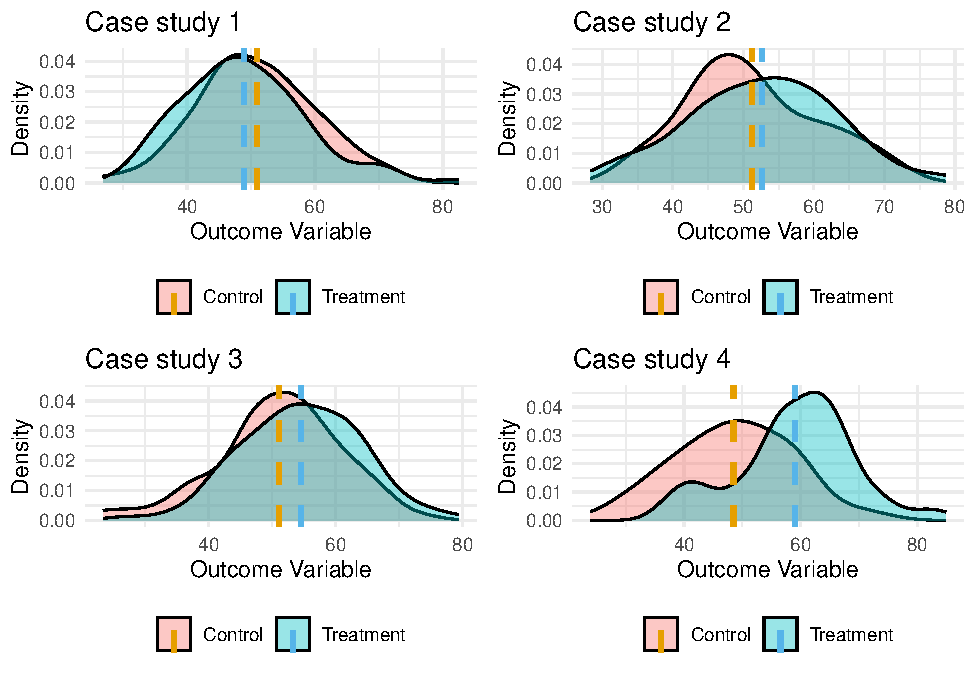
\includegraphics{_main_files/figure-latex/unnamed-chunk-1-1.pdf}

\subsection{Different Metrics for Measuring Effect Sizes}\label{different-metrics-for-measuring-effect-sizes}

Effect sizes can be calculated using a variety of metrics depending on the type of data and the comparisons being made.
Below, we present a table showing some of the most common effect size metrics, calculated for the same hypothetical data used in the visual demonstration above.

\begin{longtable}[]{@{}
  >{\raggedright\arraybackslash}p{(\columnwidth - 4\tabcolsep) * \real{0.2778}}
  >{\raggedright\arraybackslash}p{(\columnwidth - 4\tabcolsep) * \real{0.3194}}
  >{\raggedright\arraybackslash}p{(\columnwidth - 4\tabcolsep) * \real{0.4028}}@{}}
\toprule\noalign{}
\begin{minipage}[b]{\linewidth}\raggedright
\textbf{Metric}
\end{minipage} & \begin{minipage}[b]{\linewidth}\raggedright
\textbf{Formula/Definition}
\end{minipage} & \begin{minipage}[b]{\linewidth}\raggedright
\textbf{Interpretation}
\end{minipage} \\
\midrule\noalign{}
\endhead
\bottomrule\noalign{}
\endlastfoot
\textbf{Mean Difference} & Mean\_Treatment - Mean\_Control & Difference in mean values between the groups. \\
\textbf{Standardized Mean Difference (SMD)} & (Mean\_Treatment - Mean\_Control) / SD\_pooled & Cohen's \emph{d} or Hedges' \emph{g} for continuous variables. \\
\textbf{Odds Ratio (OR)} & (Odds\_Treatment / Odds\_Control) & Odds of an event occurring in the treatment vs.~control. \\
\textbf{Log Odds Ratio} & log(OR) & Stabilized variance and more symmetrical distribution. \\
\textbf{Risk Ratio (RR)} & (Risk\_Treatment / Risk\_Control) & Ratio of the probability of an event between groups. \\
\textbf{Log Risk Ratio} & log(RR) & Similar to log OR, stabilizing variances. \\
\end{longtable}

Using the simulated data above, let's compare the groups using several of these metrics:

\begin{longtable}[]{@{}
  >{\raggedright\arraybackslash}p{(\columnwidth - 8\tabcolsep) * \real{0.2000}}
  >{\raggedright\arraybackslash}p{(\columnwidth - 8\tabcolsep) * \real{0.2000}}
  >{\raggedright\arraybackslash}p{(\columnwidth - 8\tabcolsep) * \real{0.2000}}
  >{\raggedright\arraybackslash}p{(\columnwidth - 8\tabcolsep) * \real{0.2000}}
  >{\raggedright\arraybackslash}p{(\columnwidth - 8\tabcolsep) * \real{0.2000}}@{}}
\toprule\noalign{}
\begin{minipage}[b]{\linewidth}\raggedright
\textbf{Effect Size Metric}
\end{minipage} & \begin{minipage}[b]{\linewidth}\raggedright
Case study 1
\end{minipage} & \begin{minipage}[b]{\linewidth}\raggedright
\textbf{Case study 2}
\end{minipage} & \begin{minipage}[b]{\linewidth}\raggedright
Case study 3
\end{minipage} & \begin{minipage}[b]{\linewidth}\raggedright
Case study 4
\end{minipage} \\
\midrule\noalign{}
\endhead
\bottomrule\noalign{}
\endlastfoot
\end{longtable}

\begin{longtable}[]{@{}lllll@{}}
\toprule\noalign{}
\endhead
\bottomrule\noalign{}
\endlastfoot
\textbf{Mean Difference} & 0 & 3.15 & 5.27 & 7.86 \\
\end{longtable}

\begin{longtable}[]{@{}lllll@{}}
\toprule\noalign{}
\endhead
\bottomrule\noalign{}
\endlastfoot
\textbf{Standardized Mean Difference (SMD)} & 0 & 0.31 & 0.52 & 0.81 \\
\end{longtable}

\begin{longtable}[]{@{}lllll@{}}
\toprule\noalign{}
\endhead
\bottomrule\noalign{}
\endlastfoot
\textbf{Odds Ratio (OR)} & 1 & 1.28 & 1.91 & 3.75 \\
\end{longtable}

\begin{longtable}[]{@{}lllll@{}}
\toprule\noalign{}
\endhead
\bottomrule\noalign{}
\endlastfoot
\textbf{Log Odds Ratio} & 0 & 0.25 & 0.65 & 1.32 \\
\end{longtable}

\begin{longtable}[]{@{}lllll@{}}
\toprule\noalign{}
\endhead
\bottomrule\noalign{}
\endlastfoot
\textbf{Risk Ratio (RR)} & 1 & 1.18 & 1.40 & 2.25 \\
\end{longtable}

\begin{longtable}[]{@{}lllll@{}}
\toprule\noalign{}
\endhead
\bottomrule\noalign{}
\endlastfoot
\textbf{Log Risk Ratio} & 0 & 0.17 & 0.34 & 0.81 \\
\end{longtable}

These values illustrate how different metrics capture varying aspects of the comparison between groups.
We will delve into these metrics in greater detail in the next sections, exploring when and why to use each one based on your research question and data type.

Overall, effect sizes provide a powerful way to quantify the differences between groups, and choosing the appropriate metric ensures accurate and meaningful interpretations in meta-analyses and research synthesis.

\subsection{How to Measure Variability}\label{how-to-measure-variability}

Variability in effect sizes can be measured using several approaches:

\begin{itemize}
\item
  \textbf{Confidence Intervals (CIs)}: These provide a range within which the true effect size is likely to fall.
  A 95\% CI indicates that if the study were repeated many times, 95\% of the calculated intervals would contain the true effect size.
\item
  \textbf{Standard Error (SE)}: This metric quantifies the amount of variation in the effect size estimate due to sampling error.
  A smaller SE suggests that the effect size is a more reliable estimate.
\item
  \textbf{Heterogeneity Statistics}: In meta-analyses, measures like I² quantify the degree of variability among effect sizes from different studies.
  A high I² value indicates substantial variability, suggesting that differences between studies may not be due to chance alone.
\end{itemize}

\subsection{What Variability Means}\label{what-variability-means}

\begin{itemize}
\item
  \textbf{High Variability}: Suggests that the effect of the treatment varies significantly across different studies or populations.
  This could indicate that certain factors (like participant characteristics or study design) influence the effectiveness of the intervention.
\item
  \textbf{Low Variability}: Implies that the effect size is consistent across studies, leading to stronger generalizations about the treatment's effectiveness.
\end{itemize}

By understanding and measuring the variability of effect sizes, researchers can provide more nuanced interpretations of their findings and enhance the credibility of their conclusions.
This approach leads to better-informed decisions in both research and practice.

\subsection{Comparison of Effect Size and p-Value}\label{comparison-of-effect-size-and-p-value}

\textbf{Understanding the Concepts}

\begin{itemize}
\item
  \textbf{Effect Size}: This metric quantifies the magnitude of a treatment effect or the strength of an association.
  It provides a clear indication of how substantial a difference is between groups, regardless of sample size.
  A larger effect size suggests a more meaningful difference, helping researchers understand the practical significance of their findings.
\item
  \textbf{P-Value}: The p-value measures the probability that the observed results occurred by chance under the null hypothesis.
  It helps determine whether to reject the null hypothesis.
  A low p-value (typically \textless{} 0.05) indicates that the observed difference is statistically significant, but it does not inform us about the size or importance of the effect.
\end{itemize}

\textbf{Key Differences}

\begin{enumerate}
\def\labelenumi{\arabic{enumi}.}
\item
  \textbf{Focus}:

  \begin{itemize}
  \item
    \textbf{Effect Size}: Emphasizes the magnitude of the effect, providing context to the results.
  \item
    \textbf{P-Value}: Emphasizes whether the effect is statistically significant, without indicating its size.
  \end{itemize}
\item
  \textbf{Interpretation}:

  \begin{itemize}
  \item
    \textbf{Effect Size}: A high effect size indicates a strong difference, while a low effect size suggests the groups are similar.
    It informs researchers about practical implications.
  \item
    \textbf{P-Value}: A p-value tells us whether we can reject the null hypothesis.
    A significant p-value doesn't necessarily imply a large or important effect.
  \end{itemize}
\item
  \textbf{Dependence on Sample Size}:

  \begin{itemize}
  \item
    \textbf{Effect Size}: Remains stable regardless of sample size, providing a consistent measure of difference.
  \item
    \textbf{P-Value}: Can be influenced by sample size; larger samples can yield statistically significant p-values even for trivial differences.
  \end{itemize}
\end{enumerate}

\chapter{Comparative meta-analytic methods for evidence synthesis}\label{comparative-meta-analytic-methods-for-evidence-synthesis}

This chapter is designed to provide a comparative exploration of different meta-analytic approaches using the \texttt{metafor}, \texttt{meta}, and \texttt{brms} packages in R. The objective is to understand how the choice of methods (e.g., fixed-effect vs.~random-effects models) and different effect size metrics (Standardized Mean Difference, Risk Ratios, etc.) can impact the interpretation of results. We will utilize a variety of datasets to illustrate how these choices influence conclusions, highlighting key interpretative aspects when heterogeneity and study-level variations are present.

By examining multiple datasets and applying different statistical techniques, we will underscore the importance of selecting appropriate methods based on the characteristics of the data, including heterogeneity among studies and the nature of the effect sizes being analyzed.

\textbf{Prerequisites}

You should have a basic understanding of meta-analysis concepts and be familiar with R. If you haven't yet installed the necessary R packages, run the following commands:

\begin{Shaded}
\begin{Highlighting}[]
\CommentTok{\#install.packages(c("tidyverse", "metafor", "dmetar", "meta", "metadat", "ggplot2", "reactable", "ggstar", "ggpubr"))}
\end{Highlighting}
\end{Shaded}

\section{Equal-Effects Model}\label{equal-effects-model}

\subsection{Example Data}\label{example-data}

Consider the meta-analysis by Molloy et al.~(2014), which examines the relationship between conscientiousness and medication adherence. We can compute the r-to-z transformed correlation coefficient and corresponding sampling variances using the \texttt{metafor} package:

\begin{Shaded}
\begin{Highlighting}[]
\FunctionTok{library}\NormalTok{(metafor)}
\NormalTok{dat }\OtherTok{\textless{}{-}} \FunctionTok{escalc}\NormalTok{(}\AttributeTok{measure=}\StringTok{"ZCOR"}\NormalTok{, }\AttributeTok{ri=}\NormalTok{ri, }\AttributeTok{ni=}\NormalTok{ni, }\AttributeTok{data=}\NormalTok{dat.molloy2014)}
\end{Highlighting}
\end{Shaded}

The dataset contains the following columns: authors, year, sample size (ni), correlation coefficient (ri), transformed coefficient (yi), and sampling variance (vi).

\subsection{Fitting the Equal-Effects Model}\label{fitting-the-equal-effects-model}

We can fit an equal-effects model with \texttt{rma()}:

\begin{Shaded}
\begin{Highlighting}[]
\NormalTok{res.ee }\OtherTok{\textless{}{-}} \FunctionTok{rma}\NormalTok{(yi, vi, }\AttributeTok{data=}\NormalTok{dat, }\AttributeTok{method=}\StringTok{"EE"}\NormalTok{)}
\FunctionTok{summary}\NormalTok{(res.ee)}
\end{Highlighting}
\end{Shaded}

\begin{verbatim}
## 
## Equal-Effects Model (k = 16)
## 
##   logLik  deviance       AIC       BIC      AICc   
##   5.4330   38.1595   -8.8659   -8.0933   -8.5802   
## 
## I^2 (total heterogeneity / total variability):   60.69%
## H^2 (total variability / sampling variability):  2.54
## 
## Test for Heterogeneity:
## Q(df = 15) = 38.1595, p-val = 0.0009
## 
## Model Results:
## 
## estimate      se    zval    pval   ci.lb   ci.ub      
##   0.1252  0.0170  7.3642  <.0001  0.0919  0.1585  *** 
## 
## ---
## Signif. codes:  0 '***' 0.001 '**' 0.01 '*' 0.05 '.' 0.1 ' ' 1
\end{verbatim}

This outputs the estimated effect size, heterogeneity statistics (I², H²), and a test for heterogeneity.

Next, we fit the same model using \texttt{lm()} by specifying the inverse of the sampling variances as weights:

\begin{Shaded}
\begin{Highlighting}[]
\NormalTok{res.lm }\OtherTok{\textless{}{-}} \FunctionTok{lm}\NormalTok{(yi }\SpecialCharTok{\textasciitilde{}} \DecValTok{1}\NormalTok{, }\AttributeTok{weights =} \DecValTok{1}\SpecialCharTok{/}\NormalTok{vi, }\AttributeTok{data=}\NormalTok{dat)}
\FunctionTok{summary}\NormalTok{(res.lm)}
\end{Highlighting}
\end{Shaded}

\begin{verbatim}
## 
## Call:
## lm(formula = yi ~ 1, data = dat, weights = 1/vi)
## 
## Weighted Residuals:
##     Min      1Q  Median      3Q     Max 
## -3.1919 -1.0719  0.6674  1.3173  2.4695 
## 
## Coefficients:
##             Estimate Std. Error t value Pr(>|t|)    
## (Intercept)  0.12518    0.02711   4.617 0.000335 ***
## ---
## Signif. codes:  0 '***' 0.001 '**' 0.01 '*' 0.05 '.' 0.1 ' ' 1
## 
## Residual standard error: 1.595 on 15 degrees of freedom
\end{verbatim}

\subsection{Comparison of Results}\label{comparison-of-results}

\begin{enumerate}
\def\labelenumi{\arabic{enumi}.}
\item
  \textbf{Coefficient Comparison}: The estimated intercept from \texttt{lm()} matches that from \texttt{rma()}, although it's rounded differently.
\item
  \textbf{Standard Errors}: The standard error from \texttt{lm()} differs because \texttt{lm()} assumes weights are only known up to a proportionality constant (σ²e). This error can be demonstrated by extracting the estimated error variance from the \texttt{lm} object and refitting the model with \texttt{rma()}:
\end{enumerate}

\begin{Shaded}
\begin{Highlighting}[]
\FunctionTok{rma}\NormalTok{(yi, vi }\SpecialCharTok{*} \FunctionTok{sigma}\NormalTok{(res.lm)}\SpecialCharTok{\^{}}\DecValTok{2}\NormalTok{, }\AttributeTok{data=}\NormalTok{dat, }\AttributeTok{method=}\StringTok{"EE"}\NormalTok{)}
\end{Highlighting}
\end{Shaded}

\begin{verbatim}
## 
## Equal-Effects Model (k = 16)
## 
## I^2 (total heterogeneity / total variability):   0.00%
## H^2 (total variability / sampling variability):  1.00
## 
## Test for Heterogeneity:
## Q(df = 15) = 15.0000, p-val = 0.4514
## 
## Model Results:
## 
## estimate      se    zval    pval   ci.lb   ci.ub      
##   0.1252  0.0271  4.6171  <.0001  0.0720  0.1783  *** 
## 
## ---
## Signif. codes:  0 '***' 0.001 '**' 0.01 '*' 0.05 '.' 0.1 ' ' 1
\end{verbatim}

This shows that adjusting the standard errors to account for the estimated error variance results in consistent estimates across both functions.

\section{Random-Effects Model}\label{random-effects-model}

\subsection{Fitting the Random-Effects Model}\label{fitting-the-random-effects-model}

We can fit a random-effects model using \texttt{rma()} as follows:

\begin{Shaded}
\begin{Highlighting}[]
\NormalTok{res.re }\OtherTok{\textless{}{-}} \FunctionTok{rma}\NormalTok{(yi, vi, }\AttributeTok{data=}\NormalTok{dat)}
\FunctionTok{summary}\NormalTok{(res.re)}
\end{Highlighting}
\end{Shaded}

\begin{verbatim}
## 
## Random-Effects Model (k = 16; tau^2 estimator: REML)
## 
##   logLik  deviance       AIC       BIC      AICc   
##   8.6096  -17.2191  -13.2191  -11.8030  -12.2191   
## 
## tau^2 (estimated amount of total heterogeneity): 0.0081 (SE = 0.0055)
## tau (square root of estimated tau^2 value):      0.0901
## I^2 (total heterogeneity / total variability):   61.73%
## H^2 (total variability / sampling variability):  2.61
## 
## Test for Heterogeneity:
## Q(df = 15) = 38.1595, p-val = 0.0009
## 
## Model Results:
## 
## estimate      se    zval    pval   ci.lb   ci.ub      
##   0.1499  0.0316  4.7501  <.0001  0.0881  0.2118  *** 
## 
## ---
## Signif. codes:  0 '***' 0.001 '**' 0.01 '*' 0.05 '.' 0.1 ' ' 1
\end{verbatim}

Next, we try fitting the same model with the \texttt{lme()} function from the \texttt{nlme} package, specifying a variance function for fixed variances:

\begin{Shaded}
\begin{Highlighting}[]
\FunctionTok{library}\NormalTok{(nlme)}
\NormalTok{dat}\SpecialCharTok{$}\NormalTok{study }\OtherTok{\textless{}{-}} \DecValTok{1}\SpecialCharTok{:}\FunctionTok{nrow}\NormalTok{(dat)}
\NormalTok{res.lme }\OtherTok{\textless{}{-}} \FunctionTok{lme}\NormalTok{(yi }\SpecialCharTok{\textasciitilde{}} \DecValTok{1}\NormalTok{, }\AttributeTok{random =} \SpecialCharTok{\textasciitilde{}} \DecValTok{1} \SpecialCharTok{|}\NormalTok{ study, }\AttributeTok{weights =} \FunctionTok{varFixed}\NormalTok{(}\SpecialCharTok{\textasciitilde{}}\NormalTok{ vi), }\AttributeTok{data=}\NormalTok{dat)}
\FunctionTok{summary}\NormalTok{(res.lme)}
\end{Highlighting}
\end{Shaded}

\begin{verbatim}
## Linear mixed-effects model fit by REML
##   Data: dat 
##         AIC       BIC   logLik
##   -8.781569 -6.657418 7.390784
## 
## Random effects:
##  Formula: ~1 | study
##         (Intercept) Residual
## StdDev:  0.06818354 1.259548
## 
## Variance function:
##  Structure: fixed weights
##  Formula: ~vi 
## Fixed effects:  yi ~ 1 
##                 Value  Std.Error DF  t-value p-value
## (Intercept) 0.1415557 0.03071906 16 4.608073   3e-04
## 
## Standardized Within-Group Residuals:
##        Min         Q1        Med         Q3        Max 
## -1.1596768 -0.6903414  0.1964221  0.7117538  1.4616798 
## 
## Number of Observations: 16
## Number of Groups: 16
\end{verbatim}

Alternatively, we can use the \texttt{lmer()} function from the \texttt{lme4} package

\begin{Shaded}
\begin{Highlighting}[]
\FunctionTok{library}\NormalTok{(lme4)}
\NormalTok{res.lmer }\OtherTok{\textless{}{-}} \FunctionTok{lmer}\NormalTok{(yi }\SpecialCharTok{\textasciitilde{}} \DecValTok{1} \SpecialCharTok{+}\NormalTok{ (}\DecValTok{1} \SpecialCharTok{|}\NormalTok{ study), }\AttributeTok{weights =} \DecValTok{1}\SpecialCharTok{/}\NormalTok{vi, }\AttributeTok{data=}\NormalTok{dat,}
                 \AttributeTok{control=}\FunctionTok{lmerControl}\NormalTok{(}\AttributeTok{check.nobs.vs.nlev=}\StringTok{"ignore"}\NormalTok{, }\AttributeTok{check.nobs.vs.nRE=}\StringTok{"ignore"}\NormalTok{))}
\FunctionTok{summary}\NormalTok{(res.lmer)}
\end{Highlighting}
\end{Shaded}

\begin{verbatim}
## Linear mixed model fit by REML ['lmerMod']
## Formula: yi ~ 1 + (1 | study)
##    Data: dat
## Weights: 1/vi
## Control: 
## lmerControl(check.nobs.vs.nlev = "ignore", check.nobs.vs.nRE = "ignore")
## 
## REML criterion at convergence: -14.8
## 
## Scaled residuals: 
##     Min      1Q  Median      3Q     Max 
## -1.1597 -0.6903  0.1964  0.7117  1.4617 
## 
## Random effects:
##  Groups   Name        Variance Std.Dev.
##  study    (Intercept) 0.004649 0.06818 
##  Residual             1.586457 1.25955 
## Number of obs: 16, groups:  study, 16
## 
## Fixed effects:
##             Estimate Std. Error t value
## (Intercept)  0.14156    0.03072   4.608
\end{verbatim}

\subsection{Comparison of Results}\label{comparison-of-results-1}

\begin{enumerate}
\def\labelenumi{\arabic{enumi}.}
\item
  \textbf{Intercept Differences}: The estimated intercepts from \texttt{lme()} and \texttt{lmer()} differ from the estimate obtained via \texttt{rma()}.
\item
  \textbf{Standard Errors}: The standard errors, t-values, and p-values also show discrepancies for similar reasons as mentioned earlier---\texttt{lme()} and \texttt{lmer()} treat sampling variances as unknown beyond a proportionality constant.
\end{enumerate}

To illustrate, we can factor this constant into the sampling variances and refit the model with \texttt{rma()}:

\begin{Shaded}
\begin{Highlighting}[]
\FunctionTok{rma}\NormalTok{(yi, vi }\SpecialCharTok{*} \FunctionTok{sigma}\NormalTok{(res.lme)}\SpecialCharTok{\^{}}\DecValTok{2}\NormalTok{, }\AttributeTok{data=}\NormalTok{dat)}
\end{Highlighting}
\end{Shaded}

\begin{verbatim}
## 
## Random-Effects Model (k = 16; tau^2 estimator: REML)
## 
## tau^2 (estimated amount of total heterogeneity): 0.0046 (SE = 0.0049)
## tau (square root of estimated tau^2 value):      0.0682
## I^2 (total heterogeneity / total variability):   36.82%
## H^2 (total variability / sampling variability):  1.58
## 
## Test for Heterogeneity:
## Q(df = 15) = 24.0532, p-val = 0.0642
## 
## Model Results:
## 
## estimate      se    zval    pval   ci.lb   ci.ub      
##   0.1416  0.0307  4.6081  <.0001  0.0813  0.2018  *** 
## 
## ---
## Signif. codes:  0 '***' 0.001 '**' 0.01 '*' 0.05 '.' 0.1 ' ' 1
\end{verbatim}

This yields results consistent with those from \texttt{lme()}.

\subsubsection{\texorpdfstring{Comparison with the \texttt{meta} Package}{Comparison with the meta Package}}\label{comparison-with-the-meta-package}

The \texttt{meta} package provides a robust alternative for conducting meta-analyses, featuring a range of built-in functions that cater to both fixed-effect and random-effects models. This package streamlines the analysis of various effect sizes, making it accessible for researchers. For example, we can execute a meta-analysis using the \texttt{metagen()} function from the \texttt{meta} package as follows:

\begin{Shaded}
\begin{Highlighting}[]
\FunctionTok{library}\NormalTok{(meta)}
\NormalTok{res.meta }\OtherTok{\textless{}{-}} \FunctionTok{metagen}\NormalTok{(}\AttributeTok{TE =}\NormalTok{ yi, }\AttributeTok{seTE =} \FunctionTok{sqrt}\NormalTok{(vi), }\AttributeTok{data =}\NormalTok{ dat, }\AttributeTok{sm =} \StringTok{"SMD"}\NormalTok{)}
\FunctionTok{summary}\NormalTok{(res.meta)}
\end{Highlighting}
\end{Shaded}

\begin{verbatim}
##        SMD            95%-CI %W(common) %W(random)
## 1   0.1892 [-0.0011; 0.3796]        3.1        5.7
## 2   0.1634 [ 0.0917; 0.2352]       21.6       10.5
## 3   0.3541 [ 0.0823; 0.6259]        1.5        3.6
## 4   0.3316 [ 0.1395; 0.5238]        3.0        5.6
## 5   0.2769 [ 0.0409; 0.5128]        2.0        4.4
## 6   0.0000 [-0.2489; 0.2489]        1.8        4.1
## 7   0.1768 [ 0.0269; 0.3267]        4.9        7.1
## 8   0.0500 [-0.0590; 0.1591]        9.3        8.9
## 9   0.2661 [ 0.0018; 0.5304]        1.6        3.8
## 10  0.0100 [-0.0607; 0.0807]       22.2       10.6
## 11 -0.0902 [-0.3595; 0.1790]        1.5        3.7
## 12  0.3884 [ 0.1795; 0.5974]        2.5        5.1
## 13  0.0000 [-0.1844; 0.1844]        3.3        5.9
## 14  0.1511 [ 0.0663; 0.2360]       15.4       10.0
## 15  0.2448 [ 0.0873; 0.4022]        4.5        6.8
## 16  0.0400 [-0.2089; 0.2889]        1.8        4.1
## 
## Number of studies: k = 16
## 
##                         SMD           95%-CI    z  p-value
## Common effect model  0.1252 [0.0919; 0.1585] 7.36 < 0.0001
## Random effects model 0.1499 [0.0881; 0.2118] 4.75 < 0.0001
## 
## Quantifying heterogeneity:
##  tau^2 = 0.0081 [0.0017; 0.0378]; tau = 0.0901 [0.0412; 0.1944]
##  I^2 = 60.7% [32.1%; 77.2%]; H = 1.59 [1.21; 2.10]
## 
## Test of heterogeneity:
##      Q d.f. p-value
##  38.16   15  0.0009
## 
## Details on meta-analytical method:
## - Inverse variance method
## - Restricted maximum-likelihood estimator for tau^2
## - Q-Profile method for confidence interval of tau^2 and tau
\end{verbatim}

One of the key advantages of the \texttt{meta} package is its user-friendly syntax, which simplifies the process of conducting meta-analyses. Additionally, it integrates functions for visualizing results, such as forest plots, directly within its framework, enhancing the interpretability of the findings.

\subsubsection{Bayesian Meta-Analysis}\label{bayesian-meta-analysis}

Bayesian meta-analysis presents a flexible framework that accommodates the incorporation of prior distributions and quantifies uncertainty in a comprehensive manner. By employing the \texttt{brms} package, we can specify a Bayesian random-effects model as follows:

\begin{Shaded}
\begin{Highlighting}[]
\FunctionTok{library}\NormalTok{(brms)}

\CommentTok{\# Define the response variable and the standard error}
\CommentTok{\# Replace \textquotesingle{}yi\textquotesingle{} with your actual response variable and \textquotesingle{}se\textquotesingle{} with the appropriate standard error variable}
\NormalTok{response\_var }\OtherTok{\textless{}{-}} \StringTok{"yi"}  \CommentTok{\# Change this to your response variable name}
\NormalTok{se\_var }\OtherTok{\textless{}{-}} \StringTok{"sqrt(vi)"}  \CommentTok{\# Calculate the standard error (if vi is the variance)}

\CommentTok{\# Fit the Bayesian random{-}effects model with specified priors}
\NormalTok{bayes\_model }\OtherTok{\textless{}{-}} \FunctionTok{brm}\NormalTok{(}
  \AttributeTok{formula =} \FunctionTok{paste0}\NormalTok{(response\_var, }\StringTok{" | se("}\NormalTok{, se\_var, }\StringTok{") \textasciitilde{} 1 + (1 | study)"}\NormalTok{),}
  \AttributeTok{data =}\NormalTok{ dat,}
  \AttributeTok{family =}\NormalTok{ gaussian,}
  \AttributeTok{prior =} \FunctionTok{c}\NormalTok{(}
    \FunctionTok{prior}\NormalTok{(}\FunctionTok{normal}\NormalTok{(}\DecValTok{0}\NormalTok{, }\DecValTok{1}\NormalTok{), }\AttributeTok{class =} \StringTok{"Intercept"}\NormalTok{),   }\CommentTok{\# Prior for the intercept}
    \FunctionTok{prior}\NormalTok{(}\FunctionTok{cauchy}\NormalTok{(}\DecValTok{0}\NormalTok{, }\DecValTok{1}\NormalTok{), }\AttributeTok{class =} \StringTok{"sd"}\NormalTok{)            }\CommentTok{\# Prior for the standard deviation of the random effect}
\NormalTok{  ),}
  \AttributeTok{iter =} \DecValTok{200}\NormalTok{,}
  \AttributeTok{warmup =} \DecValTok{100}\NormalTok{,}
  \AttributeTok{cores =} \DecValTok{4}\NormalTok{,}
  \AttributeTok{chains =} \DecValTok{2}\NormalTok{,}
  \AttributeTok{seed =} \DecValTok{14}
\NormalTok{)}
\end{Highlighting}
\end{Shaded}

\begin{verbatim}
## Running /Library/Frameworks/R.framework/Resources/bin/R CMD SHLIB foo.c
## using C compiler: ‘Apple clang version 15.0.0 (clang-1500.3.9.4)’
## using SDK: ‘MacOSX14.4.sdk’
## clang -arch arm64 -I"/Library/Frameworks/R.framework/Resources/include" -DNDEBUG   -I"/Library/Frameworks/R.framework/Versions/4.4-arm64/Resources/library/Rcpp/include/"  -I"/Library/Frameworks/R.framework/Versions/4.4-arm64/Resources/library/RcppEigen/include/"  -I"/Library/Frameworks/R.framework/Versions/4.4-arm64/Resources/library/RcppEigen/include/unsupported"  -I"/Library/Frameworks/R.framework/Versions/4.4-arm64/Resources/library/BH/include" -I"/Library/Frameworks/R.framework/Versions/4.4-arm64/Resources/library/StanHeaders/include/src/"  -I"/Library/Frameworks/R.framework/Versions/4.4-arm64/Resources/library/StanHeaders/include/"  -I"/Library/Frameworks/R.framework/Versions/4.4-arm64/Resources/library/RcppParallel/include/"  -I"/Library/Frameworks/R.framework/Versions/4.4-arm64/Resources/library/rstan/include" -DEIGEN_NO_DEBUG  -DBOOST_DISABLE_ASSERTS  -DBOOST_PENDING_INTEGER_LOG2_HPP  -DSTAN_THREADS  -DUSE_STANC3 -DSTRICT_R_HEADERS  -DBOOST_PHOENIX_NO_VARIADIC_EXPRESSION  -D_HAS_AUTO_PTR_ETC=0  -include '/Library/Frameworks/R.framework/Versions/4.4-arm64/Resources/library/StanHeaders/include/stan/math/prim/fun/Eigen.hpp'  -D_REENTRANT -DRCPP_PARALLEL_USE_TBB=1   -I/opt/R/arm64/include    -fPIC  -falign-functions=64 -Wall -g -O2  -c foo.c -o foo.o
## In file included from <built-in>:1:
## In file included from /Library/Frameworks/R.framework/Versions/4.4-arm64/Resources/library/StanHeaders/include/stan/math/prim/fun/Eigen.hpp:22:
## In file included from /Library/Frameworks/R.framework/Versions/4.4-arm64/Resources/library/RcppEigen/include/Eigen/Dense:1:
## In file included from /Library/Frameworks/R.framework/Versions/4.4-arm64/Resources/library/RcppEigen/include/Eigen/Core:19:
## /Library/Frameworks/R.framework/Versions/4.4-arm64/Resources/library/RcppEigen/include/Eigen/src/Core/util/Macros.h:679:10: fatal error: 'cmath' file not found
## #include <cmath>
##          ^~~~~~~
## 1 error generated.
## make: *** [foo.o] Error 1
\end{verbatim}

\begin{Shaded}
\begin{Highlighting}[]
\CommentTok{\# Summarize the results}
\FunctionTok{summary}\NormalTok{(bayes\_model)}
\end{Highlighting}
\end{Shaded}

\begin{verbatim}
##  Family: gaussian 
##   Links: mu = identity; sigma = identity 
## Formula: yi | se(sqrt(vi)) ~ 1 + (1 | study) 
##    Data: dat (Number of observations: 16) 
##   Draws: 2 chains, each with iter = 200; warmup = 100; thin = 1;
##          total post-warmup draws = 200
## 
## Multilevel Hyperparameters:
## ~study (Number of levels: 16) 
##               Estimate Est.Error l-95% CI u-95% CI Rhat Bulk_ESS Tail_ESS
## sd(Intercept)     0.11      0.04     0.05     0.19 1.00       63      113
## 
## Regression Coefficients:
##           Estimate Est.Error l-95% CI u-95% CI Rhat Bulk_ESS Tail_ESS
## Intercept     0.15      0.04     0.09     0.24 1.00      180      186
## 
## Further Distributional Parameters:
##       Estimate Est.Error l-95% CI u-95% CI Rhat Bulk_ESS Tail_ESS
## sigma     0.00      0.00     0.00     0.00   NA       NA       NA
## 
## Draws were sampled using sampling(NUTS). For each parameter, Bulk_ESS
## and Tail_ESS are effective sample size measures, and Rhat is the potential
## scale reduction factor on split chains (at convergence, Rhat = 1).
## ]  (Warmup)
## Chain 2: Iteration:  80 / 200 [ 40%]  (Warmup)
## Chain 1: Iteration: 100 / 200 [ 50%]  (Warmup)
## Chain 1: Iteration: 101 / 200 [ 50%]  (Sampling)
## Chain 2: Iteration: 100 / 200 [ 50%]  (Warmup)
## Chain 2: Iteration: 101 / 200 [ 50%]  (Sampling)
## Chain 1: Iteration: 120 / 200 [ 60%]  (Sampling)
## Chain 2: Iteration: 120 / 200 [ 60%]  (Sampling)
## Chain 1: Iteration: 140 / 200 [ 70%]  (Sampling)
## Chain 2: Iteration: 140 / 200 [ 70%]  (Sampling)
## Chain 1: Iteration: 160 / 200 [ 80%]  (Sampling)
## Chain 2: Iteration: 160 / 200 [ 80%]  (Sampling)
## Chain 1: Iteration: 180 / 200 [ 90%]  (Sampling)
## Chain 2: Iteration: 180 / 200 [ 90%]  (Sampling)
## Chain 1: Iteration: 200 / 200 [100%]  (Sampling)
## Chain 1: 
## Chain 1:  Elapsed Time: 0.034 seconds (Warm-up)
## Chain 1:                0.025 seconds (Sampling)
## Chain 1:                0.059 seconds (Total)
## Chain 1: 
## Chain 2: Iteration: 200 / 200 [100%]  (Sampling)
## Chain 2: 
## Chain 2:  Elapsed Time: 0.033 seconds (Warm-up)
## Chain 2:                0.025 seconds (Sampling)
## Chain 2:                0.058 seconds (Total)
## Chain 2:
\end{verbatim}

This Bayesian approach enables us to derive posterior distributions for the effect sizes, facilitating a more nuanced interpretation of uncertainty compared to traditional frequentist methods. By leveraging Bayesian techniques, researchers can integrate prior knowledge and obtain more robust estimates, especially in cases where sample sizes are limited or when study results exhibit significant variability.

\section{Conclusion}\label{conclusion}

In summary, while the \texttt{lm()}, \texttt{lme()}, and \texttt{lmer()} functions can fit various linear models, they are not appropriate for meta-analysis due to their assumptions about the error variances. The \texttt{rma()} function is specifically designed for meta-analytic contexts, ensuring that known sampling variances are correctly utilized, resulting in reliable estimates and standard errors. Additionally, the \texttt{meta} package provides an accessible alternative for meta-analyses, while Bayesian methods using \texttt{brms} allow for flexible modeling and uncertainty quantification.

\subsection{Example 1: fixed vs.~random Meta-Analysis models}\label{example-1-fixed-vs.-random-meta-analysis-models}

\hfill\break
The first dataset explores the impact of two effect size measures: Standardized Mean Difference (SMD) and Log Risk Ratios (lnRR). We apply different models and compare the results to identify variations in interpretations:

\begin{itemize}
\tightlist
\item
  \textbf{Calculation of effect-sizes}
\end{itemize}

\begin{Shaded}
\begin{Highlighting}[]
\NormalTok{dat }\OtherTok{\textless{}{-}}\NormalTok{ metadat}\SpecialCharTok{::}\NormalTok{dat.curtis1998}

\CommentTok{\# Standardized mean differences}
\NormalTok{    SMD }\OtherTok{\textless{}{-}} \FunctionTok{escalc}\NormalTok{(}\AttributeTok{measure =} \StringTok{"SMD"}\NormalTok{, }\AttributeTok{n1i =}\NormalTok{ dat}\SpecialCharTok{$}\NormalTok{n1i, }\AttributeTok{n2i =}\NormalTok{ dat}\SpecialCharTok{$}\NormalTok{n2i, }\AttributeTok{m1i =}\NormalTok{ dat}\SpecialCharTok{$}\NormalTok{m1i, }\AttributeTok{m2i =}\NormalTok{ dat}\SpecialCharTok{$}\NormalTok{m2i, }\AttributeTok{sd1i =}\NormalTok{ dat}\SpecialCharTok{$}\NormalTok{sd1i, }\AttributeTok{sd2i =}\NormalTok{ dat}\SpecialCharTok{$}\NormalTok{sd2i)}

    \CommentTok{\# Ln(RR)}
    
\NormalTok{lnRR }\OtherTok{\textless{}{-}} \FunctionTok{escalc}\NormalTok{(}\AttributeTok{measure =} \StringTok{"ROM"}\NormalTok{, }\AttributeTok{n1i =}\NormalTok{ dat}\SpecialCharTok{$}\NormalTok{n1i, }\AttributeTok{n2i =}\NormalTok{ dat}\SpecialCharTok{$}\NormalTok{n2i, }\AttributeTok{m1i =}\NormalTok{ dat}\SpecialCharTok{$}\NormalTok{m1i, }\AttributeTok{m2i =}\NormalTok{ dat}\SpecialCharTok{$}\NormalTok{m2i, }\AttributeTok{sd1i =}\NormalTok{ dat}\SpecialCharTok{$}\NormalTok{sd1i, }\AttributeTok{sd2i =}\NormalTok{ dat}\SpecialCharTok{$}\NormalTok{sd2i)}
\end{Highlighting}
\end{Shaded}

\begin{itemize}
\tightlist
\item
  \textbf{Model Comparison:}
\end{itemize}

\begin{Shaded}
\begin{Highlighting}[]
\CommentTok{\# Fixed{-}Effect Model (SMD):}
\NormalTok{fixed\_SMD }\OtherTok{\textless{}{-}} \FunctionTok{rma}\NormalTok{(}\AttributeTok{yi =}\NormalTok{ SMD}\SpecialCharTok{$}\NormalTok{yi, }\AttributeTok{vi =}\NormalTok{ SMD}\SpecialCharTok{$}\NormalTok{vi, }\AttributeTok{method =} \StringTok{"FE"}\NormalTok{, }\AttributeTok{data =}\NormalTok{ dat)}
\NormalTok{fixed\_lnRR }\OtherTok{\textless{}{-}} \FunctionTok{rma}\NormalTok{(}\AttributeTok{yi =}\NormalTok{ lnRR}\SpecialCharTok{$}\NormalTok{yi, }\AttributeTok{vi =}\NormalTok{ lnRR}\SpecialCharTok{$}\NormalTok{vi, }\AttributeTok{method =} \StringTok{"FE"}\NormalTok{, }\AttributeTok{data =}\NormalTok{ dat)}

\CommentTok{\# random effect models }
\NormalTok{random\_m\_SMD }\OtherTok{\textless{}{-}} \FunctionTok{rma}\NormalTok{(}\AttributeTok{yi =}\NormalTok{ SMD}\SpecialCharTok{$}\NormalTok{yi, }\AttributeTok{vi =}\NormalTok{ SMD}\SpecialCharTok{$}\NormalTok{vi, }\AttributeTok{method =} \StringTok{"REML"}\NormalTok{, }\AttributeTok{data =}\NormalTok{ dat)}
\NormalTok{random\_m\_lnRR }\OtherTok{\textless{}{-}} \FunctionTok{rma}\NormalTok{(}\AttributeTok{yi =}\NormalTok{ lnRR}\SpecialCharTok{$}\NormalTok{yi, }\AttributeTok{vi =}\NormalTok{ lnRR}\SpecialCharTok{$}\NormalTok{vi, }\AttributeTok{method =} \StringTok{"REML"}\NormalTok{, }\AttributeTok{data =}\NormalTok{ dat)}
\end{Highlighting}
\end{Shaded}

\begin{itemize}
\tightlist
\item
  \textbf{Extraction and comparisons of the results}
\end{itemize}

\begin{Shaded}
\begin{Highlighting}[]
\CommentTok{\# Extract relevant results for comparison}
\NormalTok{model\_comparison }\OtherTok{\textless{}{-}} \FunctionTok{data.frame}\NormalTok{(}
  \AttributeTok{Model =} \FunctionTok{c}\NormalTok{(}\StringTok{"Fixed Effect (SMD)"}\NormalTok{, }\StringTok{"Random Effect (SMD)"}\NormalTok{, }\StringTok{"Fixed Effect (lnRR)"}\NormalTok{, }\StringTok{"Random Effect (lnRR)"}\NormalTok{),}
  \AttributeTok{Estimate =} \FunctionTok{c}\NormalTok{(fixed\_SMD}\SpecialCharTok{$}\NormalTok{b, random\_m\_SMD}\SpecialCharTok{$}\NormalTok{b, fixed\_lnRR}\SpecialCharTok{$}\NormalTok{b, random\_m\_lnRR}\SpecialCharTok{$}\NormalTok{b),}
  \StringTok{\textasciigrave{}}\AttributeTok{95\% CI Lower}\StringTok{\textasciigrave{}} \OtherTok{=} \FunctionTok{c}\NormalTok{(fixed\_SMD}\SpecialCharTok{$}\NormalTok{ci.lb, random\_m\_SMD}\SpecialCharTok{$}\NormalTok{ci.lb, fixed\_lnRR}\SpecialCharTok{$}\NormalTok{ci.lb, random\_m\_lnRR}\SpecialCharTok{$}\NormalTok{ci.lb),}
  \StringTok{\textasciigrave{}}\AttributeTok{95\% CI Upper}\StringTok{\textasciigrave{}} \OtherTok{=} \FunctionTok{c}\NormalTok{(fixed\_SMD}\SpecialCharTok{$}\NormalTok{ci.ub, random\_m\_SMD}\SpecialCharTok{$}\NormalTok{ci.ub, fixed\_lnRR}\SpecialCharTok{$}\NormalTok{ci.ub, random\_m\_lnRR}\SpecialCharTok{$}\NormalTok{ci.ub),}
  \AttributeTok{Tau2 =} \FunctionTok{c}\NormalTok{(}\ConstantTok{NA}\NormalTok{, random\_m\_SMD}\SpecialCharTok{$}\NormalTok{tau2, }\ConstantTok{NA}\NormalTok{, random\_m\_lnRR}\SpecialCharTok{$}\NormalTok{tau2),}
  \AttributeTok{I2 =} \FunctionTok{c}\NormalTok{(}\ConstantTok{NA}\NormalTok{, random\_m\_SMD}\SpecialCharTok{$}\NormalTok{I2, }\ConstantTok{NA}\NormalTok{, random\_m\_lnRR}\SpecialCharTok{$}\NormalTok{I2),}
  \AttributeTok{p.value =} \FunctionTok{c}\NormalTok{(fixed\_SMD}\SpecialCharTok{$}\NormalTok{pval, random\_m\_SMD}\SpecialCharTok{$}\NormalTok{pval, fixed\_lnRR}\SpecialCharTok{$}\NormalTok{pval, random\_m\_lnRR}\SpecialCharTok{$}\NormalTok{pval)}
\NormalTok{)}

\CommentTok{\# Affichage des résultats sous forme de tableau interactif avec reactable}
\NormalTok{model\_comparison}
\end{Highlighting}
\end{Shaded}

\begin{verbatim}
##                  Model  Estimate X95..CI.Lower X95..CI.Upper       Tau2
## 1   Fixed Effect (SMD) 1.0200088     0.9104184      1.129599         NA
## 2  Random Effect (SMD) 1.2845731     1.0619587      1.507187 0.74922116
## 3  Fixed Effect (lnRR) 0.2088297     0.1981535      0.219506         NA
## 4 Random Effect (lnRR) 0.2552978     0.2164785      0.294117 0.02620568
##         I2      p.value
## 1       NA 2.382399e-74
## 2 69.73831 1.173970e-29
## 3       NA 0.000000e+00
## 4 88.89735 5.133963e-38
\end{verbatim}

\begin{itemize}
\tightlist
\item
  \textbf{Interpretation:} The contrast in point estimates and confidence intervals between the SMD and lnRR models underscores the impact of effect size metrics on study-level variability. This comparison reveals how different metrics can shift the weight of certain studies and alter pooled estimates.
\end{itemize}

\textbf{Exercise: Model comparison}

\begin{enumerate}
\def\labelenumi{\arabic{enumi}.}
\item
  \textbf{Task}: Fit three different models (Fixed, Random, and Three-Level) using the dataset.
\item
  \textbf{Objective}: Compare their tau² estimates and overall pooled effect sizes.
\item
  \textbf{Guiding questions}:

  \begin{itemize}
  \item
    How does heterogeneity (I²) change across these models?
  \item
    Does the model choice impact the significance of moderators?
  \end{itemize}
\end{enumerate}

\subsection{Example 2: Comparing Heterogeneity across models}\label{example-2-comparing-heterogeneity-across-models}

Here, we calculate Risk Differences (RD) and explore the impact of between-study variance estimators (\texttt{DL}, \texttt{REML}) on heterogeneity.

\begin{itemize}
\tightlist
\item
  \textbf{Random-Effects Model Using DerSimonian-Laird (DL)}:
\end{itemize}

\begin{Shaded}
\begin{Highlighting}[]
\NormalTok{res\_dl }\OtherTok{\textless{}{-}} \FunctionTok{rma}\NormalTok{(}\AttributeTok{yi =}\NormalTok{ lnRR}\SpecialCharTok{$}\NormalTok{yi, }\AttributeTok{vi =}\NormalTok{ lnRR}\SpecialCharTok{$}\NormalTok{vi, }\AttributeTok{method =} \StringTok{"DL"}\NormalTok{, }\AttributeTok{data =}\NormalTok{ dat)}
\end{Highlighting}
\end{Shaded}

\begin{itemize}
\tightlist
\item
  \textbf{Random-Effects Model Using REML}:
\end{itemize}

\begin{Shaded}
\begin{Highlighting}[]
\NormalTok{res\_reml }\OtherTok{\textless{}{-}} \FunctionTok{rma}\NormalTok{(}\AttributeTok{yi =}\NormalTok{ lnRR}\SpecialCharTok{$}\NormalTok{yi, }\AttributeTok{vi =}\NormalTok{ lnRR}\SpecialCharTok{$}\NormalTok{vi, }\AttributeTok{method =} \StringTok{"REML"}\NormalTok{, }\AttributeTok{data =}\NormalTok{ dat)}
\end{Highlighting}
\end{Shaded}

\begin{itemize}
\tightlist
\item
  \textbf{Extraction and comparisons of the results}
\end{itemize}

\begin{Shaded}
\begin{Highlighting}[]
\CommentTok{\# Extract relevant results for comparison}
\NormalTok{model\_comparison2 }\OtherTok{\textless{}{-}} \FunctionTok{data.frame}\NormalTok{(}
  \AttributeTok{Model =} \FunctionTok{c}\NormalTok{(}\StringTok{"DL"}\NormalTok{, }\StringTok{"REML"}\NormalTok{),}
  \AttributeTok{Estimate =} \FunctionTok{c}\NormalTok{(res\_dl}\SpecialCharTok{$}\NormalTok{b, res\_reml}\SpecialCharTok{$}\NormalTok{b),}
  \StringTok{\textasciigrave{}}\AttributeTok{95\% CI Lower}\StringTok{\textasciigrave{}} \OtherTok{=} \FunctionTok{c}\NormalTok{(res\_dl}\SpecialCharTok{$}\NormalTok{ci.lb, res\_reml}\SpecialCharTok{$}\NormalTok{ci.lb),}
  \StringTok{\textasciigrave{}}\AttributeTok{95\% CI Upper}\StringTok{\textasciigrave{}} \OtherTok{=} \FunctionTok{c}\NormalTok{(res\_dl}\SpecialCharTok{$}\NormalTok{ci.ub, res\_reml}\SpecialCharTok{$}\NormalTok{ci.ub),}
  \AttributeTok{Tau2 =} \FunctionTok{c}\NormalTok{(res\_dl}\SpecialCharTok{$}\NormalTok{tau2, res\_reml}\SpecialCharTok{$}\NormalTok{tau2),}
  \AttributeTok{I2 =} \FunctionTok{c}\NormalTok{(res\_dl}\SpecialCharTok{$}\NormalTok{I2, res\_reml}\SpecialCharTok{$}\NormalTok{I2),}
  \AttributeTok{p.value =} \FunctionTok{c}\NormalTok{(res\_dl}\SpecialCharTok{$}\NormalTok{pval, res\_reml}\SpecialCharTok{$}\NormalTok{pval)}
\NormalTok{)}

\CommentTok{\# Affichage des résultats sous forme de tableau interactif avec reactable}
\NormalTok{model\_comparison2}
\end{Highlighting}
\end{Shaded}

\begin{verbatim}
##   Model  Estimate X95..CI.Lower X95..CI.Upper       Tau2       I2      p.value
## 1    DL 0.2530579     0.2168455     0.2892704 0.02164714 86.86638 1.065093e-42
## 2  REML 0.2552978     0.2164785     0.2941170 0.02620568 88.89735 5.133963e-38
\end{verbatim}

\textbf{Interpretation:} The DL estimator is more sensitive to small-study effects, potentially overestimating between-study heterogeneity, while the REML tends to yield more conservative estimates, resulting in narrower confidence intervals. This comparison is crucial for understanding when each method might be more appropriate.

\textbf{Exercise: Model estimator impact}

\begin{enumerate}
\def\labelenumi{\arabic{enumi}.}
\item
  \textbf{Task}: Apply multiple heterogeneity estimators (\texttt{DL}, \texttt{HE}, \texttt{SJ}, \texttt{REML}) to the dataset.
\item
  \textbf{Objective}: Compare I², tau², and Q-statistics across estimators.
\item
  \textbf{Guiding Questions}:

  \begin{itemize}
  \item
    Which estimator produces the most conservative tau² estimate?
  \item
    Does the choice of estimator affect the overall significance?
  \end{itemize}
\end{enumerate}

\subsection{Example 3: Multi-Level meta-Analysis with hierarchical Data}\label{example-3-multi-level-meta-analysis-with-hierarchical-data}

In hierarchical data structures, three-level models allow us to account for dependencies within and across clusters (e.g., experiments and individual observations).

\begin{itemize}
\tightlist
\item
  \textbf{Three-Level model setup}:
\end{itemize}

\begin{Shaded}
\begin{Highlighting}[]
\NormalTok{dat}\OtherTok{\textless{}{-}}\FunctionTok{cbind}\NormalTok{(dat, lnRR)}
\CommentTok{\# Three{-}level meta{-}analysis}
\NormalTok{three\_level\_m }\OtherTok{\textless{}{-}} \FunctionTok{rma.mv}\NormalTok{(}\AttributeTok{yi =}\NormalTok{ yi, }\AttributeTok{V =}\NormalTok{ vi, }\AttributeTok{random =} \FunctionTok{list}\NormalTok{(}\SpecialCharTok{\textasciitilde{}}\DecValTok{1} \SpecialCharTok{|}\NormalTok{ id, }\SpecialCharTok{\textasciitilde{}}\DecValTok{1} \SpecialCharTok{|}\NormalTok{ paper), }\AttributeTok{data =}\NormalTok{ dat)}

\CommentTok{\# Two level meta{-}analysis}
\NormalTok{two\_level\_m }\OtherTok{\textless{}{-}} \FunctionTok{rma.mv}\NormalTok{(}\AttributeTok{yi =}\NormalTok{ yi, }\AttributeTok{V =}\NormalTok{ vi, }\AttributeTok{random =} \FunctionTok{list}\NormalTok{(}\SpecialCharTok{\textasciitilde{}}\DecValTok{1} \SpecialCharTok{|}\NormalTok{ id), }\AttributeTok{data =}\NormalTok{ dat)}
\end{Highlighting}
\end{Shaded}

\begin{enumerate}
\def\labelenumi{\arabic{enumi}.}
\tightlist
\item
  Faire le tableau de comparaison de outputs
\item
  AIC pour sélection de modèles
\end{enumerate}

\textbf{Interpretation:} The three-level model reveals the extent of within- and between-experiment variance. Visualizing these results with orchard plots helps disentangle which levels contribute most to the observed heterogeneity.

\textbf{Exercise: multi-Level meta-Analysis}

\begin{enumerate}
\def\labelenumi{\arabic{enumi}.}
\item
  \textbf{Task}: Fit a series of multi-level models with different group-level random effects.
\item
  \textbf{Objective}: Determine how accounting for more complex structures impacts model fit and tau² partitioning.
\item
  \textbf{Guiding Questions}:

  \begin{itemize}
  \item
    How does the inclusion of nested random effects change the intraclass correlation?
  \item
    Which levels (experiment vs.~within-group) contribute most to the variance?
  \end{itemize}
\end{enumerate}

\subsection{Model Selection in Meta-Analysis}\label{model-selection-in-meta-analysis}

Choosing the best model in meta-analysis involves comparing multiple competing models using selection criteria like AIC (Akaike Information Criterion), AICc (Corrected AIC), BIC (Bayesian Information Criterion), and other model performance metrics. This helps identify a model that balances goodness-of-fit and model complexity. The following section covers strategies for selecting the most appropriate model, including fixed and random effects, based on theoretical knowledge or statistical tests.

\subsubsection{\texorpdfstring{\textbf{Selection Criteria for Model Comparison}}{Selection Criteria for Model Comparison}}\label{selection-criteria-for-model-comparison}

\begin{itemize}
\item
  \textbf{AIC (Akaike Information Criterion)}: Measures the trade-off between model fit and complexity:

  \[
  \text{AIC} = 2k - 2\log(\hat{L})
  \]

  where \(k\) is the number of model parameters, and \(\hat{L}\) is the maximum likelihood value. A lower AIC indicates a more parsimonious model.
\item
  \textbf{AICc (Corrected AIC)}: Adjusted for small sample sizes to avoid overfitting:

  \[
  \text{AICc} = \text{AIC} + \frac{2k(k+1)}{n - k - 1}
  \]

  It should be used when \(n/k\) is small (\textless{} 40), where \(n\) is the number of observations and \(k\) the number of parameters.
\item
  \textbf{BIC (Bayesian Information Criterion)}: Applies a stronger penalty for the number of parameters:

  \[
  \text{BIC} = k\log(n) - 2\log(\hat{L})
  \]

  BIC often favors simpler models, making it suitable when working with large sample sizes.
\item
  \textbf{Likelihood Ratio Tests and ANOVA}: To directly compare nested models, likelihood ratio tests or \texttt{anova} can be used. This approach quantifies if adding (or removing) parameters significantly improves model fit.
\end{itemize}

\subsubsection{\texorpdfstring{\textbf{Choosing Between Fixed and Random-Effects Models}}{Choosing Between Fixed and Random-Effects Models}}\label{choosing-between-fixed-and-random-effects-models}

The decision between using a fixed-effect or random-effects model depends on either \emph{theoretical considerations} or \emph{statistical testing}:

\begin{itemize}
\item
  \textbf{Theoretical Justification}: Choose a \emph{fixed-effect model} if you expect a common effect size across all studies (e.g., homogeneous study contexts or interventions). Select a \emph{random-effects model} when heterogeneity among studies is anticipated (e.g., varying contexts, differing methods).
\item
  \textbf{Statistical Testing}:

  \begin{itemize}
  \tightlist
  \item
    \textbf{Heterogeneity Tests}: Use tests like Cochran's Q-test or \(I^2\) statistics to detect significant variability between studies. High \(I^2\) or a significant Q-test indicates that a random-effects model is likely more appropriate.
  \item
    \textbf{ANOVA for Model Comparison}: When comparing nested models (e.g., fixed-effects vs.~random-effects), \texttt{anova()} can be used to test whether the inclusion of random effects significantly improves the model fit.
  \end{itemize}
\item
\end{itemize}

\subsubsection{\texorpdfstring{\textbf{Comparing Models: Fixed and Random Structures}}{Comparing Models: Fixed and Random Structures}}\label{comparing-models-fixed-and-random-structures}

When fitting mixed-effects models, choosing between different random and fixed structures is a crucial step. Typically, the process involves:

\begin{enumerate}
\def\labelenumi{\arabic{enumi}.}
\item
  \textbf{Start with the Random Structure}:

  \begin{itemize}
  \item
    Define the random effects first to capture variance due to grouping or clustering (e.g., study-level random effects, site-level random effects).
  \item
    Use the likelihood ratio test (\texttt{anova()}) to compare models with and without each random component:

\begin{Shaded}
\begin{Highlighting}[]
\NormalTok{model1 }\OtherTok{\textless{}{-}} \FunctionTok{rma.mv}\NormalTok{(yi, vi, }\AttributeTok{random =} \SpecialCharTok{\textasciitilde{}} \DecValTok{1} \SpecialCharTok{|}\NormalTok{ paper, }\AttributeTok{data =}\NormalTok{ dat)}
\NormalTok{model2 }\OtherTok{\textless{}{-}} \FunctionTok{rma.mv}\NormalTok{(yi, vi, }\AttributeTok{random =} \SpecialCharTok{\textasciitilde{}} \DecValTok{1} \SpecialCharTok{|}\NormalTok{ paper}\SpecialCharTok{/}\NormalTok{id, }\AttributeTok{data =}\NormalTok{ dat)}
\FunctionTok{anova}\NormalTok{(model1, model2)}
\end{Highlighting}
\end{Shaded}

\begin{verbatim}
## 
##         df      AIC      BIC     AICc   logLik      LRT   pval       QE 
## Full     3  -8.2204  -0.3750  -7.9730   7.1102                 769.0185 
## Reduced  2 104.0570 109.2872 104.1794 -50.0285 114.2774 <.0001 769.0185
\end{verbatim}
  \end{itemize}

  This step allows you to determine if additional random components (e.g., study vs.~nested study/site effects) are justified.

  Here, \texttt{anova()} will test if the more complex model (\texttt{model\_random}) explains significantly more variance than the simpler one (\texttt{model\_fixed}).
\item
  \textbf{Incorporate Fixed Effects}:

  \begin{itemize}
  \item
    After selecting the optimal random structure, test different combinations of fixed effects (e.g., covariates, moderators).
  \item
    Compare models using AIC, AICc, and BIC. Include one fixed effect at a time and use \texttt{anova()} to see if adding predictors improves fit:

\begin{Shaded}
\begin{Highlighting}[]
\NormalTok{model\_fixed1 }\OtherTok{\textless{}{-}} \FunctionTok{rma.mv}\NormalTok{(yi, vi, }\AttributeTok{mods =} \SpecialCharTok{\textasciitilde{}}\NormalTok{ species, }\AttributeTok{random=} \SpecialCharTok{\textasciitilde{}} \DecValTok{1} \SpecialCharTok{|}\NormalTok{ paper}\SpecialCharTok{/}\NormalTok{id, }\AttributeTok{data =}\NormalTok{ dat)}
\NormalTok{model\_fixed2 }\OtherTok{\textless{}{-}} \FunctionTok{rma.mv}\NormalTok{(yi, vi, }\AttributeTok{mods =} \SpecialCharTok{\textasciitilde{}}\NormalTok{ species }\SpecialCharTok{+}\NormalTok{ fungrp,}\AttributeTok{random=} \SpecialCharTok{\textasciitilde{}} \DecValTok{1} \SpecialCharTok{|}\NormalTok{ paper}\SpecialCharTok{/}\NormalTok{id, }\AttributeTok{data =}\NormalTok{ dat)}
\FunctionTok{anova}\NormalTok{(model\_fixed1, model\_fixed2)}
\end{Highlighting}
\end{Shaded}

\begin{verbatim}
## 
##         df     AIC      BIC     AICc logLik    LRT   pval       QE 
## Full    38 73.7811 156.9879 183.5588 1.1095               334.3528 
## Reduced 37 71.3274 152.9011 168.2930 1.3363 0.0000 1.0000 334.9388
\end{verbatim}
  \end{itemize}
\item
  \textbf{Test for Interactions}:

  \begin{itemize}
  \tightlist
  \item
    After defining main effects, consider adding interaction terms and use AIC or likelihood ratio tests to assess their contribution.
  \end{itemize}
\end{enumerate}

\subsubsection{\texorpdfstring{\textbf{Selecting the Optimal Model: Practical Considerations}}{Selecting the Optimal Model: Practical Considerations}}\label{selecting-the-optimal-model-practical-considerations}

\begin{itemize}
\tightlist
\item
  \textbf{Model Complexity vs.~Parsimony}: Start with a simple model and gradually add parameters, using AIC, AICc, and BIC to avoid overfitting.
\item
  \textbf{Check Model Assumptions}: Ensure that the chosen model meets meta-analytic assumptions (e.g., homogeneity of variance, normality).
\item
  \textbf{Visual Evaluation}: Use diagnostic plots (e.g., residual plots, forest plots) to visually inspect model fit.
\end{itemize}

In practice, the ideal strategy involves:

\begin{enumerate}
\def\labelenumi{\arabic{enumi}.}
\tightlist
\item
  \textbf{Define the Random Structure First}:

  \begin{itemize}
  \tightlist
  \item
    Use theoretical and statistical justifications to select between study-level or multi-level random effects.
  \item
    Select the most parsimonious random structure using \texttt{anova()} and AIC/BIC.
  \end{itemize}
\item
  \textbf{Add Fixed Effects Incrementally}:

  \begin{itemize}
  \tightlist
  \item
    Start with primary predictors and gradually include covariates, using \texttt{anova()} to compare nested models.
  \item
    Check for interactions only after establishing main effects.
  \end{itemize}
\item
  \textbf{Assess the Final Model}:

  \begin{itemize}
  \tightlist
  \item
    Compare the best candidate models (fixed vs.~random) using AIC, AICc, BIC, and likelihood ratio tests.
  \item
    Select the model that balances fit and interpretability.
  \end{itemize}
\end{enumerate}

This structured approach ensures that both theoretical considerations and statistical criteria are employed for robust model selection in meta-analyses.

\chapter{Analysing model variability}\label{analysing-model-variability}

\subsection{Using Parametric and Non-Parametric Bootstrapping to Estimate Confidence Intervals in Meta-Analyses}\label{using-parametric-and-non-parametric-bootstrapping-to-estimate-confidence-intervals-in-meta-analyses}

\textbf{Bootstrapping} is a statistical technique used to estimate the sampling distribution of an estimator by repeatedly resampling from the observed data. In meta-analysis, bootstrapping is commonly applied to construct more robust confidence intervals (CIs) for parameters such as the overall effect size (μ\muμ) and the between-study variance (τ2\tau\^{}2τ2). This chapter will demonstrate how to implement both parametric and non-parametric bootstrapping methods using the \texttt{boot} package in R, emphasizing best practices for obtaining reliable results.

\subsection{Overview}\label{overview}

\begin{itemize}
\item
  \textbf{Parametric Bootstrapping}: Assumes a specific distributional form for the data (e.g., normal distribution of residuals). The data are generated based on parameter estimates from the fitted model.
\item
  \textbf{Non-Parametric Bootstrapping}: Does not rely on specific distributional assumptions. The bootstrap samples are created directly by resampling the original data with replacement.
\end{itemize}

\subsection{Parametric Bootstrapping: Step-by-Step Example}\label{parametric-bootstrapping-step-by-step-example}

In parametric bootstrapping, we generate new datasets by simulating values from a specified distribution using the parameter estimates from the fitted model. This process requires defining two functions:

\begin{enumerate}
\def\labelenumi{\arabic{enumi}.}
\item
  A function to compute the statistics of interest (e.g., the mean effect size μ\muμ and the between-study variance τ2\tau\^{}2τ2) based on the bootstrap data.
\item
  A function to generate the bootstrap datasets.
\end{enumerate}

Let's illustrate this approach with a random-effects model:

\textbf{Defining the Function}

The function \texttt{boot.func()} calculates the effect size and variance components based on each bootstrap dataset:

\begin{Shaded}
\begin{Highlighting}[]
\CommentTok{\# Load necessary libraries}
\FunctionTok{library}\NormalTok{(metafor)}
\FunctionTok{library}\NormalTok{(boot)}


\CommentTok{\# 1. Fit the initial random{-}effects model}
\NormalTok{initial\_model }\OtherTok{\textless{}{-}} \FunctionTok{rma}\NormalTok{(yi, vi, }\AttributeTok{data=}\NormalTok{dat)}

\CommentTok{\# Extract estimated parameters for later use}
\NormalTok{mu\_estimate }\OtherTok{\textless{}{-}} \FunctionTok{coef}\NormalTok{(initial\_model)}
\NormalTok{tau2\_estimate }\OtherTok{\textless{}{-}}\NormalTok{ initial\_model}\SpecialCharTok{$}\NormalTok{tau2}

\CommentTok{\# 2. Define the Statistic Function for Bootstrapping}
\NormalTok{boot.func }\OtherTok{\textless{}{-}} \ControlFlowTok{function}\NormalTok{(data.boot) \{}
  \CommentTok{\# Fit the random{-}effects model to the bootstrap data}
\NormalTok{  res }\OtherTok{\textless{}{-}} \FunctionTok{try}\NormalTok{(}\FunctionTok{suppressWarnings}\NormalTok{(}\FunctionTok{rma}\NormalTok{(yi, vi, }\AttributeTok{data=}\NormalTok{data.boot)), }\AttributeTok{silent=}\ConstantTok{TRUE}\NormalTok{)}
  
  \CommentTok{\# Return NA if the model did not converge}
  \ControlFlowTok{if}\NormalTok{ (}\FunctionTok{inherits}\NormalTok{(res, }\StringTok{"try{-}error"}\NormalTok{)) \{}
    \FunctionTok{return}\NormalTok{(}\FunctionTok{rep}\NormalTok{(}\ConstantTok{NA}\NormalTok{, }\DecValTok{4}\NormalTok{))  }\CommentTok{\# Return a vector of NAs}
\NormalTok{  \} }\ControlFlowTok{else}\NormalTok{ \{}
    \CommentTok{\# Extract the estimated effect size (mu), its variance, tau², and its variance}
    \FunctionTok{return}\NormalTok{(}\FunctionTok{c}\NormalTok{(}\FunctionTok{coef}\NormalTok{(res), }\FunctionTok{diag}\NormalTok{(}\FunctionTok{vcov}\NormalTok{(res)), res}\SpecialCharTok{$}\NormalTok{tau2, res}\SpecialCharTok{$}\NormalTok{se.tau2}\SpecialCharTok{\^{}}\DecValTok{2}\NormalTok{))}
\NormalTok{  \}}
\NormalTok{\}}

\CommentTok{\# 3. Define the Data Generation Function for Bootstrapping}
\NormalTok{data.gen }\OtherTok{\textless{}{-}} \ControlFlowTok{function}\NormalTok{(dat, mle) \{}
  \CommentTok{\# Generate effect sizes based on the estimated mu and tau²}
  \FunctionTok{data.frame}\NormalTok{(}\AttributeTok{yi =} \FunctionTok{rnorm}\NormalTok{(}\FunctionTok{nrow}\NormalTok{(dat), mle}\SpecialCharTok{$}\NormalTok{mu, }\FunctionTok{sqrt}\NormalTok{(mle}\SpecialCharTok{$}\NormalTok{tau2 }\SpecialCharTok{+}\NormalTok{ dat}\SpecialCharTok{$}\NormalTok{vi)), }\AttributeTok{vi =}\NormalTok{ dat}\SpecialCharTok{$}\NormalTok{vi)}
\NormalTok{\}}

\CommentTok{\# 4. Running the Parametric Bootstrap}
\FunctionTok{set.seed}\NormalTok{(}\DecValTok{1234}\NormalTok{)  }\CommentTok{\# For reproducibility}
\NormalTok{res.boot }\OtherTok{\textless{}{-}}\NormalTok{ boot}\SpecialCharTok{::}\FunctionTok{boot}\NormalTok{(dat, }
                        \AttributeTok{statistic =}\NormalTok{ boot.func, }
                        \AttributeTok{R =} \DecValTok{100}\NormalTok{, }
                        \AttributeTok{sim =} \StringTok{"parametric"}\NormalTok{, }
                        \AttributeTok{ran.gen =}\NormalTok{ data.gen, }
                        \AttributeTok{mle =} \FunctionTok{list}\NormalTok{(}\AttributeTok{mu =}\NormalTok{ mu\_estimate, }\AttributeTok{tau2 =}\NormalTok{ tau2\_estimate))}

\CommentTok{\# Check results}
\FunctionTok{print}\NormalTok{(res.boot)}
\end{Highlighting}
\end{Shaded}

\begin{verbatim}
## 
## PARAMETRIC BOOTSTRAP
## 
## 
## Call:
## boot::boot(data = dat, statistic = boot.func, R = 100, sim = "parametric", 
##     ran.gen = data.gen, mle = list(mu = mu_estimate, tau2 = tau2_estimate))
## 
## 
## Bootstrap Statistics :
##         original        bias     std. error
## t1* 2.552978e-01  1.086396e-03 1.908634e-02
## t2* 3.922816e-04 -9.255823e-06 5.149671e-05
## t3* 2.620568e-02 -7.892906e-04 4.629509e-03
## t4* 2.819226e-05 -8.527037e-07 7.784439e-06
\end{verbatim}

\textbf{Extracting Confidence Intervals}

After running the bootstrap, we can calculate the confidence intervals for the mean effect size (μ\muμ) and the between-study variance (τ2\tau\^{}2τ2) using different bootstrap methods (normal, basic, studentized, percentile):

\begin{Shaded}
\begin{Highlighting}[]
\CommentTok{\# Confidence intervals for mu}
\FunctionTok{boot.ci}\NormalTok{(res.boot, }\AttributeTok{type=}\FunctionTok{c}\NormalTok{(}\StringTok{"norm"}\NormalTok{, }\StringTok{"basic"}\NormalTok{, }\StringTok{"stud"}\NormalTok{, }\StringTok{"perc"}\NormalTok{), }\AttributeTok{index=}\DecValTok{1}\SpecialCharTok{:}\DecValTok{2}\NormalTok{)}
\end{Highlighting}
\end{Shaded}

\begin{verbatim}
## BOOTSTRAP CONFIDENCE INTERVAL CALCULATIONS
## Based on 100 bootstrap replicates
## 
## CALL : 
## boot.ci(boot.out = res.boot, type = c("norm", "basic", "stud", 
##     "perc"), index = 1:2)
## 
## Intervals : 
## Level      Normal              Basic         
## 95%   ( 0.2168,  0.2916 )   ( 0.2137,  0.2933 )  
## 
## Level    Studentized          Percentile     
## 95%   ( 0.2123,  0.2956 )   ( 0.2173,  0.2969 )  
## Calculations and Intervals on Original Scale
## Some basic intervals may be unstable
## Some studentized intervals may be unstable
## Some percentile intervals may be unstable
\end{verbatim}

\begin{Shaded}
\begin{Highlighting}[]
\CommentTok{\# Confidence intervals for tau²}
\FunctionTok{boot.ci}\NormalTok{(res.boot, }\AttributeTok{type=}\FunctionTok{c}\NormalTok{(}\StringTok{"norm"}\NormalTok{, }\StringTok{"basic"}\NormalTok{, }\StringTok{"stud"}\NormalTok{, }\StringTok{"perc"}\NormalTok{), }\AttributeTok{index=}\DecValTok{3}\SpecialCharTok{:}\DecValTok{4}\NormalTok{)}
\end{Highlighting}
\end{Shaded}

\begin{verbatim}
## BOOTSTRAP CONFIDENCE INTERVAL CALCULATIONS
## Based on 100 bootstrap replicates
## 
## CALL : 
## boot.ci(boot.out = res.boot, type = c("norm", "basic", "stud", 
##     "perc"), index = 3:4)
## 
## Intervals : 
## Level      Normal              Basic         
## 95%   ( 0.0179,  0.0361 )   ( 0.0160,  0.0373 )  
## 
## Level    Studentized          Percentile     
## 95%   ( 0.0184,  0.0432 )   ( 0.0152,  0.0364 )  
## Calculations and Intervals on Original Scale
## Some basic intervals may be unstable
## Some studentized intervals may be unstable
## Some percentile intervals may be unstable
\end{verbatim}

These commands compute CIs based on various bootstrap methods, allowing comparison of the interval estimates.

\subsection{Non-Parametric Bootstrapping: Step-by-Step Example}\label{non-parametric-bootstrapping-step-by-step-example}

Non-parametric bootstrapping involves generating new datasets by resampling the original data with replacement. We only need to define a single function for this purpose:

\textbf{Defining the Function}

\begin{Shaded}
\begin{Highlighting}[]
\CommentTok{\# Load necessary libraries}
\FunctionTok{library}\NormalTok{(metafor)}
\FunctionTok{library}\NormalTok{(boot)}


\CommentTok{\# 1. Fit the initial random{-}effects model}
\NormalTok{initial\_model }\OtherTok{\textless{}{-}} \FunctionTok{rma}\NormalTok{(yi, vi, }\AttributeTok{data=}\NormalTok{dat)}

\CommentTok{\# Extract estimated parameters for later use}
\NormalTok{mu\_estimate }\OtherTok{\textless{}{-}} \FunctionTok{coef}\NormalTok{(initial\_model)}
\NormalTok{tau2\_estimate }\OtherTok{\textless{}{-}}\NormalTok{ initial\_model}\SpecialCharTok{$}\NormalTok{tau2}

\CommentTok{\# 2. Define the Statistic Function for Bootstrapping}
\NormalTok{boot.func }\OtherTok{\textless{}{-}} \ControlFlowTok{function}\NormalTok{(data.boot, indices) \{}
   \CommentTok{\# Resample the data based on the given indices}
\NormalTok{   sel }\OtherTok{\textless{}{-}}\NormalTok{ data.boot[indices, ]}
   
   \CommentTok{\# Fit the random{-}effects model to the resampled data}
\NormalTok{   res }\OtherTok{\textless{}{-}} \FunctionTok{try}\NormalTok{(}\FunctionTok{suppressWarnings}\NormalTok{(}\FunctionTok{rma}\NormalTok{(yi, vi, }\AttributeTok{data=}\NormalTok{sel)), }\AttributeTok{silent=}\ConstantTok{TRUE}\NormalTok{)}
   
   \CommentTok{\# Return NA if the model did not converge}
   \ControlFlowTok{if}\NormalTok{ (}\FunctionTok{inherits}\NormalTok{(res, }\StringTok{"try{-}error"}\NormalTok{)) \{}
      \FunctionTok{return}\NormalTok{(}\FunctionTok{rep}\NormalTok{(}\ConstantTok{NA}\NormalTok{, }\DecValTok{4}\NormalTok{))  }\CommentTok{\# Return a vector of NAs}
\NormalTok{   \} }\ControlFlowTok{else}\NormalTok{ \{}
      \CommentTok{\# Extract the estimated effect size (mu), its variance, tau², and its variance}
      \FunctionTok{return}\NormalTok{(}\FunctionTok{c}\NormalTok{(}\FunctionTok{coef}\NormalTok{(res), }\FunctionTok{diag}\NormalTok{(}\FunctionTok{vcov}\NormalTok{(res)), res}\SpecialCharTok{$}\NormalTok{tau2, res}\SpecialCharTok{$}\NormalTok{se.tau2}\SpecialCharTok{\^{}}\DecValTok{2}\NormalTok{))}
\NormalTok{   \}}
\NormalTok{\}}

\CommentTok{\# 3. Define the Data Generation Function for Bootstrapping}
\NormalTok{data.gen }\OtherTok{\textless{}{-}} \ControlFlowTok{function}\NormalTok{(dat, mle) \{}
   \CommentTok{\# Generate effect sizes based on the estimated mu and tau²}
   \FunctionTok{data.frame}\NormalTok{(}\AttributeTok{yi =} \FunctionTok{rnorm}\NormalTok{(}\FunctionTok{nrow}\NormalTok{(dat), mle}\SpecialCharTok{$}\NormalTok{mu, }\FunctionTok{sqrt}\NormalTok{(mle}\SpecialCharTok{$}\NormalTok{tau2 }\SpecialCharTok{+}\NormalTok{ dat}\SpecialCharTok{$}\NormalTok{vi)), }\AttributeTok{vi =}\NormalTok{ dat}\SpecialCharTok{$}\NormalTok{vi)}
\NormalTok{\}}

\CommentTok{\# 4. Running the Parametric Bootstrap}
\FunctionTok{set.seed}\NormalTok{(}\DecValTok{1234}\NormalTok{)  }\CommentTok{\# For reproducibility}
\NormalTok{res.boot }\OtherTok{\textless{}{-}}\NormalTok{ boot}\SpecialCharTok{::}\FunctionTok{boot}\NormalTok{(dat, }
                        \AttributeTok{statistic =}\NormalTok{ boot.func, }
                        \AttributeTok{R =} \DecValTok{100}\NormalTok{, }
                        \AttributeTok{sim =} \StringTok{"parametric"}\NormalTok{, }
                        \AttributeTok{ran.gen =}\NormalTok{ data.gen, }
                        \AttributeTok{mle =} \FunctionTok{list}\NormalTok{(}\AttributeTok{mu =}\NormalTok{ mu\_estimate, }\AttributeTok{tau2 =}\NormalTok{ tau2\_estimate))}

\CommentTok{\# Check results}
\FunctionTok{print}\NormalTok{(res.boot)}
\end{Highlighting}
\end{Shaded}

\begin{verbatim}
## 
## PARAMETRIC BOOTSTRAP
## 
## 
## Call:
## boot::boot(data = dat, statistic = boot.func, R = 100, sim = "parametric", 
##     ran.gen = data.gen, mle = list(mu = mu_estimate, tau2 = tau2_estimate))
## 
## 
## Bootstrap Statistics :
##         original        bias     std. error
## t1* 2.552978e-01  1.086396e-03 1.908634e-02
## t2* 3.922816e-04 -9.255823e-06 5.149671e-05
## t3* 2.620568e-02 -7.892906e-04 4.629509e-03
## t4* 2.819226e-05 -8.527037e-07 7.784439e-06
\end{verbatim}

\textbf{Extracting Confidence Intervals}

After running the bootstrap, we can calculate the confidence intervals for the mean effect size (μ\muμ) and the between-study variance (τ2\tau\^{}2τ2) using different bootstrap methods (normal, basic, studentized, percentile):

\begin{Shaded}
\begin{Highlighting}[]
\CommentTok{\# Confidence intervals for mu}
\FunctionTok{boot.ci}\NormalTok{(res.boot, }\AttributeTok{type=}\FunctionTok{c}\NormalTok{(}\StringTok{"norm"}\NormalTok{, }\StringTok{"basic"}\NormalTok{, }\StringTok{"stud"}\NormalTok{, }\StringTok{"perc"}\NormalTok{), }\AttributeTok{index=}\DecValTok{1}\SpecialCharTok{:}\DecValTok{2}\NormalTok{)}
\end{Highlighting}
\end{Shaded}

\begin{verbatim}
## BOOTSTRAP CONFIDENCE INTERVAL CALCULATIONS
## Based on 100 bootstrap replicates
## 
## CALL : 
## boot.ci(boot.out = res.boot, type = c("norm", "basic", "stud", 
##     "perc"), index = 1:2)
## 
## Intervals : 
## Level      Normal              Basic         
## 95%   ( 0.2168,  0.2916 )   ( 0.2137,  0.2933 )  
## 
## Level    Studentized          Percentile     
## 95%   ( 0.2123,  0.2956 )   ( 0.2173,  0.2969 )  
## Calculations and Intervals on Original Scale
## Some basic intervals may be unstable
## Some studentized intervals may be unstable
## Some percentile intervals may be unstable
\end{verbatim}

\begin{Shaded}
\begin{Highlighting}[]
\CommentTok{\# Confidence intervals for tau²}
\FunctionTok{boot.ci}\NormalTok{(res.boot, }\AttributeTok{type=}\FunctionTok{c}\NormalTok{(}\StringTok{"norm"}\NormalTok{, }\StringTok{"basic"}\NormalTok{, }\StringTok{"stud"}\NormalTok{, }\StringTok{"perc"}\NormalTok{), }\AttributeTok{index=}\DecValTok{3}\SpecialCharTok{:}\DecValTok{4}\NormalTok{)}
\end{Highlighting}
\end{Shaded}

\begin{verbatim}
## BOOTSTRAP CONFIDENCE INTERVAL CALCULATIONS
## Based on 100 bootstrap replicates
## 
## CALL : 
## boot.ci(boot.out = res.boot, type = c("norm", "basic", "stud", 
##     "perc"), index = 3:4)
## 
## Intervals : 
## Level      Normal              Basic         
## 95%   ( 0.0179,  0.0361 )   ( 0.0160,  0.0373 )  
## 
## Level    Studentized          Percentile     
## 95%   ( 0.0184,  0.0432 )   ( 0.0152,  0.0364 )  
## Calculations and Intervals on Original Scale
## Some basic intervals may be unstable
## Some studentized intervals may be unstable
## Some percentile intervals may be unstable
\end{verbatim}

\textbf{Comparing Bootstrap Methods}

The choice between parametric and non-parametric bootstrapping depends on the underlying assumptions and the sample size:

\begin{itemize}
\item
  \textbf{Parametric Bootstrapping} is more appropriate when we have strong assumptions about the distribution of effect sizes.
\item
  \textbf{Non-Parametric Bootstrapping} is recommended when the sample size is relatively small or when we want to avoid making strict assumptions.
\end{itemize}

\textbf{Visualization of Bootstrap Distributions}

To visualize the bootstrap distributions, we can create kernel density plots to inspect the variability and shape of the bootstrap samples:

\begin{Shaded}
\begin{Highlighting}[]
\CommentTok{\# Visualize the bootstrap distribution for mu}
\FunctionTok{plot}\NormalTok{(}\FunctionTok{density}\NormalTok{(res.boot}\SpecialCharTok{$}\NormalTok{t[,}\DecValTok{1}\NormalTok{]), }\AttributeTok{main=}\StringTok{"Bootstrap Distribution of Mu"}\NormalTok{)}
\FunctionTok{abline}\NormalTok{(}\AttributeTok{v=}\FunctionTok{quantile}\NormalTok{(res.boot}\SpecialCharTok{$}\NormalTok{t[,}\DecValTok{1}\NormalTok{], }\AttributeTok{probs=}\FunctionTok{c}\NormalTok{(}\FloatTok{0.025}\NormalTok{, }\FloatTok{0.975}\NormalTok{)), }\AttributeTok{col=}\StringTok{"red"}\NormalTok{)}
\end{Highlighting}
\end{Shaded}

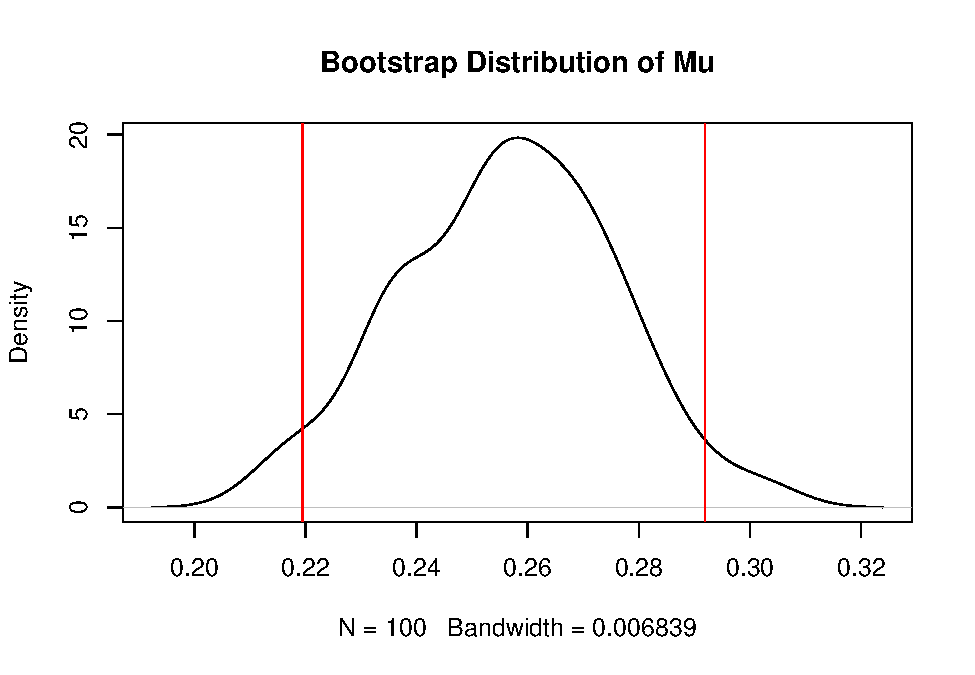
\includegraphics{_main_files/figure-latex/unnamed-chunk-27-1.pdf}

\subsection{Conclusion}\label{conclusion-1}

Bootstrapping provides a flexible and powerful method for estimating confidence intervals in meta-analysis. However, it is important to consider potential issues such as non-convergence of models during the bootstrap process, as well as the assumptions underlying each method. When applying bootstrap methods, carefully evaluate the coverage of different interval types and compare the results to standard methods (e.g., Wald-type CIs or Knapp-Hartung adjustments).

In the next section, we will delve deeper into \textbf{prediction intervals}, which provide a complementary measure of uncertainty, reflecting the variability in effect sizes for new studies.

\chapter{Plotting meta-analytical results}\label{plotting-meta-analytical-results}

\subsection{Overview}\label{overview-1}

This chapter focuses on the visualization of meta-analytical results, which is crucial for effectively communicating findings and insights drawn from aggregated data. Visualization techniques help researchers and stakeholders quickly grasp complex relationships and patterns within the data. In this chapter, we will cover various plotting methods, including forest plots, funnel plots, and advanced visualizations using R packages such as \texttt{ggplot2}, \texttt{metafor}, and \texttt{dmetar}.

\subsection{Example 1: Forest plot with metafor}\label{example-1-forest-plot-with-metafor}

\begin{Shaded}
\begin{Highlighting}[]
\NormalTok{dat }\OtherTok{\textless{}{-}} \FunctionTok{data.frame}\NormalTok{(}\AttributeTok{author =} \FunctionTok{c}\NormalTok{(}\StringTok{"Dyson"}\NormalTok{, }\StringTok{"Jönsson"}\NormalTok{, }\StringTok{"Morris"}\NormalTok{, }\StringTok{"Saslow"}\NormalTok{, }\StringTok{"Saslow"}\NormalTok{, }\StringTok{"Sato"}\NormalTok{, }\StringTok{"Tay"}\NormalTok{, }\StringTok{"Yamada"}\NormalTok{),}
                  \AttributeTok{year   =} \FunctionTok{c}\NormalTok{(}\DecValTok{2010}\NormalTok{, }\DecValTok{2009}\NormalTok{, }\DecValTok{2019}\NormalTok{, }\DecValTok{2014}\NormalTok{, }\DecValTok{2017}\NormalTok{, }\DecValTok{2017}\NormalTok{, }\DecValTok{2014}\NormalTok{, }\DecValTok{2014}\NormalTok{),}
                  \AttributeTok{ai     =} \FunctionTok{c}\NormalTok{(}\DecValTok{3}\NormalTok{, }\DecValTok{6}\NormalTok{, }\DecValTok{11}\NormalTok{, }\DecValTok{8}\NormalTok{, }\DecValTok{6}\NormalTok{, }\DecValTok{4}\NormalTok{, }\DecValTok{36}\NormalTok{, }\DecValTok{2}\NormalTok{), }\DocumentationTok{\#\#Nb event experimental group}
                  \AttributeTok{n1i    =} \FunctionTok{c}\NormalTok{(}\DecValTok{6}\NormalTok{, }\DecValTok{6}\NormalTok{, }\DecValTok{21}\NormalTok{, }\DecValTok{9}\NormalTok{, }\DecValTok{11}\NormalTok{, }\DecValTok{22}\NormalTok{, }\DecValTok{46}\NormalTok{, }\DecValTok{12}\NormalTok{), }\DocumentationTok{\#\# Total experimental group}
                  \AttributeTok{ci     =} \FunctionTok{c}\NormalTok{(}\DecValTok{1}\NormalTok{, }\DecValTok{3}\NormalTok{, }\DecValTok{0}\NormalTok{, }\DecValTok{5}\NormalTok{, }\DecValTok{0}\NormalTok{, }\DecValTok{0}\NormalTok{, }\DecValTok{30}\NormalTok{, }\DecValTok{2}\NormalTok{),  }\DocumentationTok{\#\# Nb events control group}
                  \AttributeTok{n2i    =} \FunctionTok{c}\NormalTok{(}\DecValTok{6}\NormalTok{, }\DecValTok{6}\NormalTok{, }\DecValTok{12}\NormalTok{, }\DecValTok{13}\NormalTok{, }\DecValTok{8}\NormalTok{, }\DecValTok{27}\NormalTok{, }\DecValTok{47}\NormalTok{, }\DecValTok{12}\NormalTok{))  }\DocumentationTok{\#\# Total control group}

\DocumentationTok{\#\#\# calculate risk differences and corresponding sampling variances (and use}
\DocumentationTok{\#\#\# the \textquotesingle{}slab\textquotesingle{} argument to store study labels as part of the data frame)}
\NormalTok{dat }\OtherTok{\textless{}{-}} \FunctionTok{escalc}\NormalTok{(}\AttributeTok{measure =} \StringTok{"RD"}\NormalTok{, }\AttributeTok{ai =}\NormalTok{ ai, }\AttributeTok{n1i =}\NormalTok{ n1i, }\AttributeTok{ci =}\NormalTok{ ci, }\AttributeTok{n2i =}\NormalTok{ n2i, }\AttributeTok{data =}\NormalTok{ dat,}
              \AttributeTok{slab =} \FunctionTok{paste}\NormalTok{(}\StringTok{" "}\NormalTok{, author, year), }\AttributeTok{addyi =} \ConstantTok{FALSE}\NormalTok{)}

\DocumentationTok{\#\#\# fit random{-}effects model (using the DL estimator)}
\NormalTok{res }\OtherTok{\textless{}{-}} \FunctionTok{rma}\NormalTok{(yi, vi, }\AttributeTok{data =}\NormalTok{ dat, }\AttributeTok{method =} \StringTok{"DL"}\NormalTok{)}

\DocumentationTok{\#\#\# colors to be used in the plot}
\NormalTok{colp }\OtherTok{\textless{}{-}} \StringTok{"\#6b58a6"}
\NormalTok{coll }\OtherTok{\textless{}{-}} \StringTok{"\#a7a9ac"}

\DocumentationTok{\#\#\# total number of studies}
\NormalTok{k }\OtherTok{\textless{}{-}} \FunctionTok{nrow}\NormalTok{(dat)}

\DocumentationTok{\#\#\# generate point sizes}
\NormalTok{psize }\OtherTok{\textless{}{-}} \FunctionTok{weights}\NormalTok{(res)}
\NormalTok{psize }\OtherTok{\textless{}{-}} \FloatTok{1.2} \SpecialCharTok{+}\NormalTok{ (psize }\SpecialCharTok{{-}} \FunctionTok{min}\NormalTok{(psize)) }\SpecialCharTok{/}\NormalTok{ (}\FunctionTok{max}\NormalTok{(psize) }\SpecialCharTok{{-}} \FunctionTok{min}\NormalTok{(psize))}

\DocumentationTok{\#\#\# get the weights and format them as will be used in the forest plot}
\NormalTok{weights }\OtherTok{\textless{}{-}} \FunctionTok{round}\NormalTok{(}\FunctionTok{weights}\NormalTok{(res), }\DecValTok{1}\NormalTok{)}

\DocumentationTok{\#\#\# adjust the margins}
\FunctionTok{par}\NormalTok{(}\AttributeTok{mar =} \FunctionTok{c}\NormalTok{(}\FloatTok{2.7}\NormalTok{, }\FloatTok{3.2}\NormalTok{, }\FloatTok{2.3}\NormalTok{, }\FloatTok{1.3}\NormalTok{), }\AttributeTok{mgp =} \FunctionTok{c}\NormalTok{(}\DecValTok{3}\NormalTok{, }\DecValTok{0}\NormalTok{, }\DecValTok{0}\NormalTok{), }\AttributeTok{tcl =} \FloatTok{0.15}\NormalTok{)}

\DocumentationTok{\#\#\# forest plot with extra annotations}
\NormalTok{sav }\OtherTok{\textless{}{-}} \FunctionTok{forest}\NormalTok{(dat}\SpecialCharTok{$}\NormalTok{yi, dat}\SpecialCharTok{$}\NormalTok{vi, }\AttributeTok{xlim =} \FunctionTok{c}\NormalTok{(}\SpecialCharTok{{-}}\FloatTok{3.4}\NormalTok{, }\FloatTok{2.1}\NormalTok{), }\AttributeTok{ylim =} \FunctionTok{c}\NormalTok{(}\SpecialCharTok{{-}}\FloatTok{0.5}\NormalTok{, k }\SpecialCharTok{+} \DecValTok{3}\NormalTok{), }\AttributeTok{alim =} \FunctionTok{c}\NormalTok{(}\SpecialCharTok{{-}}\DecValTok{1}\NormalTok{, }\DecValTok{1}\NormalTok{), }\AttributeTok{cex =} \FloatTok{0.88}\NormalTok{,}
              \AttributeTok{pch =} \DecValTok{18}\NormalTok{, }\AttributeTok{psize =}\NormalTok{ psize, }\AttributeTok{efac =} \DecValTok{0}\NormalTok{, }\AttributeTok{refline =} \ConstantTok{NA}\NormalTok{, }\AttributeTok{lty =} \FunctionTok{c}\NormalTok{(}\DecValTok{1}\NormalTok{, }\DecValTok{0}\NormalTok{), }\AttributeTok{xlab =} \StringTok{""}\NormalTok{,}
              \AttributeTok{ilab =} \FunctionTok{cbind}\NormalTok{(}\FunctionTok{paste}\NormalTok{(dat}\SpecialCharTok{$}\NormalTok{ai, }\StringTok{"/"}\NormalTok{, dat}\SpecialCharTok{$}\NormalTok{n1i), }\FunctionTok{paste}\NormalTok{(dat}\SpecialCharTok{$}\NormalTok{ci, }\StringTok{"/"}\NormalTok{, dat}\SpecialCharTok{$}\NormalTok{n2i), weights),}
              \AttributeTok{ilab.xpos =} \FunctionTok{c}\NormalTok{(}\SpecialCharTok{{-}}\FloatTok{1.9}\NormalTok{, }\SpecialCharTok{{-}}\FloatTok{1.3}\NormalTok{, }\FloatTok{1.2}\NormalTok{), }\AttributeTok{annosym =} \FunctionTok{c}\NormalTok{(}\StringTok{" ("}\NormalTok{, }\StringTok{" to "}\NormalTok{, }\StringTok{")"}\NormalTok{),}
              \AttributeTok{rowadj =} \SpecialCharTok{{-}}\FloatTok{0.07}\NormalTok{)}

\DocumentationTok{\#\#\# add the vertical reference line at 0}
\FunctionTok{segments}\NormalTok{(}\DecValTok{0}\NormalTok{, }\SpecialCharTok{{-}}\DecValTok{1}\NormalTok{, }\DecValTok{0}\NormalTok{, k }\SpecialCharTok{+} \FloatTok{1.6}\NormalTok{, }\AttributeTok{col =}\NormalTok{ coll)}

\DocumentationTok{\#\#\# add the vertical reference line at the pooled estimate}
\FunctionTok{segments}\NormalTok{(}\FunctionTok{coef}\NormalTok{(res), }\DecValTok{0}\NormalTok{, }\FunctionTok{coef}\NormalTok{(res), k, }\AttributeTok{col =}\NormalTok{ colp, }\AttributeTok{lty =} \StringTok{"33"}\NormalTok{, }\AttributeTok{lwd =} \FloatTok{0.8}\NormalTok{)}

\DocumentationTok{\#\#\# redraw the CI lines and points in the chosen color}
\FunctionTok{segments}\NormalTok{(}\FunctionTok{summary}\NormalTok{(dat)}\SpecialCharTok{$}\NormalTok{ci.lb, k}\SpecialCharTok{:}\DecValTok{1}\NormalTok{, }\FunctionTok{summary}\NormalTok{(dat)}\SpecialCharTok{$}\NormalTok{ci.ub, k}\SpecialCharTok{:}\DecValTok{1}\NormalTok{, }\AttributeTok{col =}\NormalTok{ colp, }\AttributeTok{lwd =} \FloatTok{1.5}\NormalTok{)}
\FunctionTok{points}\NormalTok{(dat}\SpecialCharTok{$}\NormalTok{yi, k}\SpecialCharTok{:}\DecValTok{1}\NormalTok{, }\AttributeTok{pch =} \DecValTok{18}\NormalTok{, }\AttributeTok{cex =}\NormalTok{ psize }\SpecialCharTok{*} \FloatTok{1.15}\NormalTok{, }\AttributeTok{col =} \StringTok{"white"}\NormalTok{)}
\FunctionTok{points}\NormalTok{(dat}\SpecialCharTok{$}\NormalTok{yi, k}\SpecialCharTok{:}\DecValTok{1}\NormalTok{, }\AttributeTok{pch =} \DecValTok{18}\NormalTok{, }\AttributeTok{cex =}\NormalTok{ psize, }\AttributeTok{col =}\NormalTok{ colp)}

\DocumentationTok{\#\#\# add the summary polygon}
\FunctionTok{addpoly}\NormalTok{(res, }\AttributeTok{row =} \DecValTok{0}\NormalTok{, }\AttributeTok{mlab =} \StringTok{"Total (95\% CI)"}\NormalTok{, }\AttributeTok{efac =} \DecValTok{2}\NormalTok{, }\AttributeTok{col =}\NormalTok{ colp, }\AttributeTok{border =}\NormalTok{ colp)}

\DocumentationTok{\#\#\# add the horizontal line at the top}
\FunctionTok{abline}\NormalTok{(}\AttributeTok{h =}\NormalTok{ k }\SpecialCharTok{+} \FloatTok{1.6}\NormalTok{, }\AttributeTok{col =}\NormalTok{ coll)}

\DocumentationTok{\#\#\# redraw the x{-}axis in the chosen color}
\FunctionTok{axis}\NormalTok{(}\AttributeTok{side =} \DecValTok{1}\NormalTok{, }\AttributeTok{at =} \FunctionTok{seq}\NormalTok{(}\SpecialCharTok{{-}}\DecValTok{1}\NormalTok{, }\DecValTok{1}\NormalTok{, }\AttributeTok{by =} \FloatTok{0.5}\NormalTok{), }\AttributeTok{col =}\NormalTok{ coll, }\AttributeTok{labels =} \ConstantTok{FALSE}\NormalTok{)}

\DocumentationTok{\#\#\# now we add a bunch of text; since some of the text falls outside of the}
\DocumentationTok{\#\#\# plot region, we set xpd=NA so nothing gets clipped}
\FunctionTok{par}\NormalTok{(}\AttributeTok{xpd =} \ConstantTok{NA}\NormalTok{)}

\DocumentationTok{\#\#\# adjust cex as used in the forest plot and use a bold font}
\FunctionTok{par}\NormalTok{(}\AttributeTok{cex =}\NormalTok{ sav}\SpecialCharTok{$}\NormalTok{cex, }\AttributeTok{font =} \DecValTok{2}\NormalTok{)}

\DocumentationTok{\#\#\# add headings}
\FunctionTok{text}\NormalTok{(sav}\SpecialCharTok{$}\NormalTok{xlim[}\DecValTok{1}\NormalTok{], k }\SpecialCharTok{+} \FloatTok{2.5}\NormalTok{, }\AttributeTok{pos =} \DecValTok{4}\NormalTok{, }\StringTok{"Study or}\SpecialCharTok{\textbackslash{}n}\StringTok{subgroup"}\NormalTok{)}
\FunctionTok{text}\NormalTok{(}\FunctionTok{mean}\NormalTok{(sav}\SpecialCharTok{$}\NormalTok{ilab.xpos[}\DecValTok{1}\SpecialCharTok{:}\DecValTok{2}\NormalTok{]), k }\SpecialCharTok{+} \FloatTok{3.4}\NormalTok{, }\StringTok{"No of events / total"}\NormalTok{)}
\FunctionTok{text}\NormalTok{(}\DecValTok{0}\NormalTok{, k }\SpecialCharTok{+} \FloatTok{2.7}\NormalTok{, }\StringTok{"Risk difference, IV,}\SpecialCharTok{\textbackslash{}n}\StringTok{random (95\% CI)"}\NormalTok{)}
\FunctionTok{text}\NormalTok{(}\FunctionTok{c}\NormalTok{(sav}\SpecialCharTok{$}\NormalTok{ilab.xpos[}\DecValTok{3}\NormalTok{], sav}\SpecialCharTok{$}\NormalTok{xlim[}\DecValTok{2}\NormalTok{] }\SpecialCharTok{{-}} \FloatTok{0.35}\NormalTok{), k }\SpecialCharTok{+} \FloatTok{2.7}\NormalTok{, }\FunctionTok{c}\NormalTok{(}\StringTok{"Weight}\SpecialCharTok{\textbackslash{}n}\StringTok{(\%)"}\NormalTok{, }\StringTok{"Risk difference, IV,}\SpecialCharTok{\textbackslash{}n}\StringTok{random (95\% CI)"}\NormalTok{))}

\DocumentationTok{\#\#\# add \textquotesingle{}Favours control\textquotesingle{}/\textquotesingle{}Favours experimental\textquotesingle{} text below the x{-}axis}
\FunctionTok{text}\NormalTok{(}\FunctionTok{c}\NormalTok{(}\SpecialCharTok{{-}}\DecValTok{1}\NormalTok{, }\DecValTok{1}\NormalTok{), }\SpecialCharTok{{-}}\FloatTok{2.5}\NormalTok{, }\FunctionTok{c}\NormalTok{(}\StringTok{"Favors control"}\NormalTok{, }\StringTok{"Favors experimental"}\NormalTok{), }\AttributeTok{pos =} \FunctionTok{c}\NormalTok{(}\DecValTok{4}\NormalTok{, }\DecValTok{2}\NormalTok{), }\AttributeTok{offset =} \SpecialCharTok{{-}}\FloatTok{0.3}\NormalTok{)}

\DocumentationTok{\#\#\# use a non{-}bold font for the rest of the text}
\FunctionTok{par}\NormalTok{(}\AttributeTok{cex =}\NormalTok{ sav}\SpecialCharTok{$}\NormalTok{cex, }\AttributeTok{font =} \DecValTok{1}\NormalTok{)}

\DocumentationTok{\#\#\# add text with heterogeneity statistics}
\FunctionTok{text}\NormalTok{(sav}\SpecialCharTok{$}\NormalTok{xlim[}\DecValTok{1}\NormalTok{], }\SpecialCharTok{{-}}\DecValTok{1}\NormalTok{, }\AttributeTok{pos =} \DecValTok{4}\NormalTok{, }\FunctionTok{bquote}\NormalTok{(}\FunctionTok{paste}\NormalTok{(}\StringTok{"Test for heterogeneity: "}\NormalTok{,}
\NormalTok{                                          tau}\SpecialCharTok{\^{}}\DecValTok{2}\NormalTok{, }\StringTok{"="}\NormalTok{, .(}\FunctionTok{round}\NormalTok{(res}\SpecialCharTok{$}\NormalTok{tau2, }\AttributeTok{digits =} \DecValTok{2}\NormalTok{)), }\StringTok{"; "}\NormalTok{,}
\NormalTok{                                          I}\SpecialCharTok{\^{}}\DecValTok{2}\NormalTok{, }\StringTok{"="}\NormalTok{, .(}\FunctionTok{round}\NormalTok{(res}\SpecialCharTok{$}\NormalTok{I2, }\AttributeTok{digits =} \DecValTok{2}\NormalTok{)), }\StringTok{"\%"}\NormalTok{)))}

\DocumentationTok{\#\#\# add text with overall estimate}
\FunctionTok{text}\NormalTok{(sav}\SpecialCharTok{$}\NormalTok{xlim[}\DecValTok{1}\NormalTok{], }\SpecialCharTok{{-}}\FloatTok{2.5}\NormalTok{, }\AttributeTok{pos =} \DecValTok{4}\NormalTok{, }\FunctionTok{bquote}\NormalTok{(}\FunctionTok{paste}\NormalTok{(}\StringTok{"Overall effect: "}\NormalTok{,}
\NormalTok{                                              riskdiff }\SpecialCharTok{==}\NormalTok{ .(}\FunctionTok{round}\NormalTok{(}\FunctionTok{coef}\NormalTok{(res), }\AttributeTok{digits =} \DecValTok{2}\NormalTok{)))))}

\DocumentationTok{\#\#\# add titles}
\FunctionTok{text}\NormalTok{(sav}\SpecialCharTok{$}\NormalTok{xlim[}\DecValTok{1}\NormalTok{], k }\SpecialCharTok{+} \FloatTok{4.5}\NormalTok{, }\AttributeTok{pos =} \DecValTok{4}\NormalTok{, }\StringTok{"Risk difference between low and very low carbohydrate diets"}\NormalTok{)}
\end{Highlighting}
\end{Shaded}

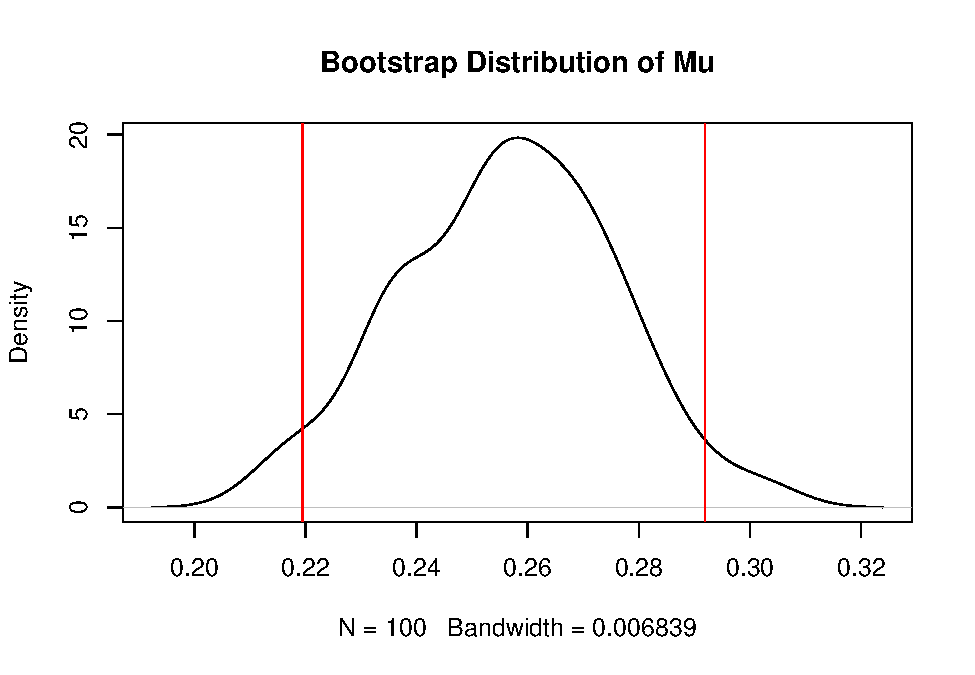
\includegraphics{_main_files/figure-latex/unnamed-chunk-28-1.pdf}

\subsection{Example 2: Forest plot with meta}\label{example-2-forest-plot-with-meta}

\begin{Shaded}
\begin{Highlighting}[]
\FunctionTok{library}\NormalTok{(meta)}
\CommentTok{\# Perform meta{-}analysis using the metagen function from \textasciigrave{}meta\textasciigrave{}}
\CommentTok{\# Perform meta{-}analysis using the metagen function from \textasciigrave{}meta\textasciigrave{}}
\NormalTok{meta\_analysis }\OtherTok{\textless{}{-}} \FunctionTok{metagen}\NormalTok{(}
  \AttributeTok{TE =}\NormalTok{ dat}\SpecialCharTok{$}\NormalTok{yi,  }\CommentTok{\# Use the calculated effect sizes}
  \AttributeTok{seTE =} \FunctionTok{sqrt}\NormalTok{(dat}\SpecialCharTok{$}\NormalTok{vi),  }\CommentTok{\# Standard errors}
  \AttributeTok{studlab =} \FunctionTok{paste}\NormalTok{(dat}\SpecialCharTok{$}\NormalTok{author, dat}\SpecialCharTok{$}\NormalTok{year),}
  \AttributeTok{data =}\NormalTok{ dat,}
  \AttributeTok{sm =} \StringTok{"RD"}\NormalTok{,  }\CommentTok{\# Risk Difference as the summary measure}
  \AttributeTok{fixed =} \ConstantTok{FALSE}\NormalTok{,  }\CommentTok{\# Using a random{-}effects model}
  \AttributeTok{random =} \ConstantTok{TRUE}\NormalTok{,}
  \AttributeTok{method.tau =} \StringTok{"REML"}\NormalTok{,  }\CommentTok{\# Restricted maximum likelihood estimator}
  \AttributeTok{hakn =} \ConstantTok{TRUE}\NormalTok{,  }\CommentTok{\# Knapp{-}Hartung adjustment}
  \AttributeTok{title =} \StringTok{"Risk Difference between Diet Groups"}
\NormalTok{)}

\CommentTok{\# Create a forest plot with custom options and store the output}
\NormalTok{forest\_plot }\OtherTok{\textless{}{-}}\NormalTok{ meta}\SpecialCharTok{::}\FunctionTok{forest}\NormalTok{(}
\NormalTok{  meta\_analysis,}
  \AttributeTok{prediction =} \ConstantTok{TRUE}\NormalTok{,  }\CommentTok{\# Add a prediction interval}
  \AttributeTok{print.tau2 =} \ConstantTok{TRUE}\NormalTok{,  }\CommentTok{\# Print the tau{-}squared statistic in the plot}
  \AttributeTok{leftlabs =} \FunctionTok{c}\NormalTok{(}\StringTok{"Study"}\NormalTok{, }\StringTok{"Risk Diff"}\NormalTok{, }\StringTok{"Std. Error"}\NormalTok{),  }\CommentTok{\# Custom labels}
  \AttributeTok{lab.e =} \StringTok{"Favours Low Carb"}\NormalTok{,  }\CommentTok{\# Label for experimental group}
  \AttributeTok{lab.c =} \StringTok{"Favours Control"}\NormalTok{,  }\CommentTok{\# Label for control group}
  \AttributeTok{col.study =} \StringTok{"\#6b58a6"}\NormalTok{,  }\CommentTok{\# Study point color}
  \AttributeTok{col.diamond =} \StringTok{"\#5e84c0"}\NormalTok{,  }\CommentTok{\# Color of the summary diamond}
  \AttributeTok{col.square =} \StringTok{"white"}  \CommentTok{\# Color for individual study estimates}
\NormalTok{)}

\FunctionTok{library}\NormalTok{(grid)}
\FunctionTok{grid.text}\NormalTok{(}\StringTok{"Meta{-}analysis of Risk Differences in Diet Studies"}\NormalTok{, }
          \AttributeTok{x =} \FloatTok{0.5}\NormalTok{, }\AttributeTok{y =} \FunctionTok{unit}\NormalTok{(}\FloatTok{0.95}\NormalTok{, }\StringTok{"npc"}\NormalTok{), }
          \AttributeTok{gp =} \FunctionTok{gpar}\NormalTok{(}\AttributeTok{fontsize =} \DecValTok{14}\NormalTok{, }\AttributeTok{fontface =} \StringTok{"bold"}\NormalTok{))}
\FunctionTok{grid.text}\NormalTok{(}\StringTok{"Random{-}effects model with Knapp{-}Hartung adjustments"}\NormalTok{, }
          \AttributeTok{x =} \FloatTok{0.5}\NormalTok{, }\AttributeTok{y =} \FunctionTok{unit}\NormalTok{(}\FloatTok{0.93}\NormalTok{, }\StringTok{"npc"}\NormalTok{), }
          \AttributeTok{gp =} \FunctionTok{gpar}\NormalTok{(}\AttributeTok{fontsize =} \DecValTok{12}\NormalTok{))}
\end{Highlighting}
\end{Shaded}

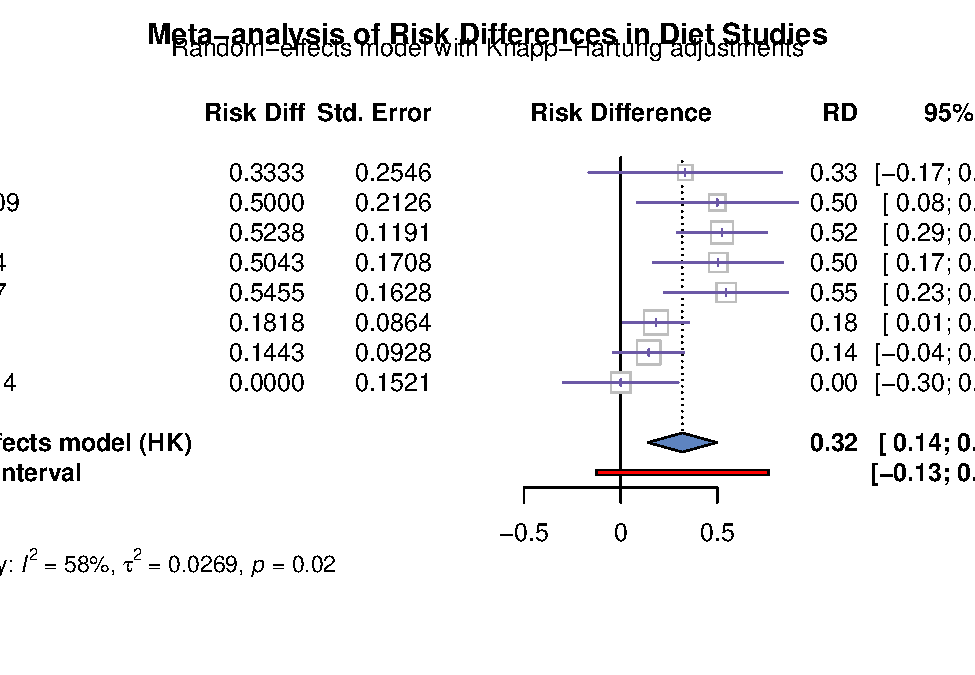
\includegraphics{_main_files/figure-latex/unnamed-chunk-29-1.pdf}

\subsection{Example 3: Forest plot with ggplot}\label{example-3-forest-plot-with-ggplot}

\begin{Shaded}
\begin{Highlighting}[]
\CommentTok{\# Load necessary libraries}
\FunctionTok{library}\NormalTok{(ggplot2)}
\FunctionTok{library}\NormalTok{(dplyr)}
\FunctionTok{library}\NormalTok{(ggpubr)}
\end{Highlighting}
\end{Shaded}

\begin{verbatim}
## 
## Attaching package: 'ggpubr'
\end{verbatim}

\begin{verbatim}
## The following object is masked from 'package:cowplot':
## 
##     get_legend
\end{verbatim}

\begin{Shaded}
\begin{Highlighting}[]
\FunctionTok{library}\NormalTok{(ggstar)}

\CommentTok{\# Prepare the data: Calculate estimates, confidence intervals, and other metrics}
\NormalTok{dat }\OtherTok{\textless{}{-}}\NormalTok{ dat }\SpecialCharTok{\%\textgreater{}\%}
  \FunctionTok{mutate}\NormalTok{(}
    \AttributeTok{estimate =}\NormalTok{ yi,  }\CommentTok{\# Estimated effect size}
    \AttributeTok{conf.low =}\NormalTok{ yi }\SpecialCharTok{{-}} \FloatTok{1.96} \SpecialCharTok{*} \FunctionTok{sqrt}\NormalTok{(vi),  }\CommentTok{\# Lower bound of the confidence interval}
    \AttributeTok{conf.high =}\NormalTok{ yi }\SpecialCharTok{+} \FloatTok{1.96} \SpecialCharTok{*} \FunctionTok{sqrt}\NormalTok{(vi),  }\CommentTok{\# Upper bound of the confidence interval}
    \AttributeTok{Sub\_Cat\_intervention =} \FunctionTok{paste}\NormalTok{(author, year)  }\CommentTok{\# Combine author and year for labels}
\NormalTok{  )}

\CommentTok{\# Create a ggplot forest plot}
\NormalTok{p }\OtherTok{\textless{}{-}} \FunctionTok{ggplot}\NormalTok{(dat, }\FunctionTok{aes}\NormalTok{(estimate, }\FunctionTok{reorder}\NormalTok{(Sub\_Cat\_intervention, estimate))) }\SpecialCharTok{+}
  \CommentTok{\# Add stars for effect sizes}
  \FunctionTok{geom\_star}\NormalTok{(}\AttributeTok{starshape =} \DecValTok{12}\NormalTok{, }\AttributeTok{size =} \DecValTok{4}\NormalTok{, }\AttributeTok{starstroke =} \FloatTok{1.1}\NormalTok{, }\AttributeTok{color =} \StringTok{"\#6b58a6"}\NormalTok{) }\SpecialCharTok{+}
  \CommentTok{\# Add points for individual study estimates}
  \FunctionTok{geom\_point}\NormalTok{(}\FunctionTok{aes}\NormalTok{(}\AttributeTok{size =}\NormalTok{ n1i), }\AttributeTok{shape =} \DecValTok{21}\NormalTok{, }\AttributeTok{alpha =} \FloatTok{0.8}\NormalTok{, }\AttributeTok{fill =} \StringTok{"\#ff9d02"}\NormalTok{,}
             \AttributeTok{position =} \FunctionTok{position\_dodge}\NormalTok{(}\AttributeTok{width =} \FloatTok{0.6}\NormalTok{)) }\SpecialCharTok{+}
  \CommentTok{\# Add error bars using confidence intervals}
  \FunctionTok{geom\_errorbar}\NormalTok{(}\FunctionTok{aes}\NormalTok{(}\AttributeTok{xmin =}\NormalTok{ conf.low, }\AttributeTok{xmax =}\NormalTok{ conf.high), }\AttributeTok{color =} \StringTok{"black"}\NormalTok{,}
                \AttributeTok{size =} \FloatTok{0.2}\NormalTok{, }\AttributeTok{width =} \FloatTok{0.1}\NormalTok{) }\SpecialCharTok{+}
  \CommentTok{\# Add a vertical line at x = 0}
  \FunctionTok{geom\_vline}\NormalTok{(}\AttributeTok{xintercept =} \DecValTok{0}\NormalTok{, }\AttributeTok{linetype =} \DecValTok{2}\NormalTok{, }\AttributeTok{color =} \StringTok{"gray"}\NormalTok{) }\SpecialCharTok{+}
  \CommentTok{\# Apply ggpubr theme}
  \FunctionTok{theme\_pubr}\NormalTok{() }\SpecialCharTok{+}
  \CommentTok{\# Set x{-}axis limits}
  \FunctionTok{xlim}\NormalTok{(}\FunctionTok{c}\NormalTok{(}\SpecialCharTok{{-}}\FloatTok{3.5}\NormalTok{, }\FloatTok{3.5}\NormalTok{)) }\SpecialCharTok{+}  \CommentTok{\# Adjust limits based on your data}
  \CommentTok{\# Remove legend}
  \FunctionTok{theme}\NormalTok{(}\AttributeTok{legend.position =} \StringTok{"none"}\NormalTok{) }\SpecialCharTok{+}
  \CommentTok{\# Set axis labels}
  \FunctionTok{labs}\NormalTok{(}\AttributeTok{y =} \StringTok{""}\NormalTok{, }\AttributeTok{x =} \StringTok{"Risk Difference (RD)"}\NormalTok{)}

\CommentTok{\# Display the plot}
\FunctionTok{print}\NormalTok{(p)}
\end{Highlighting}
\end{Shaded}

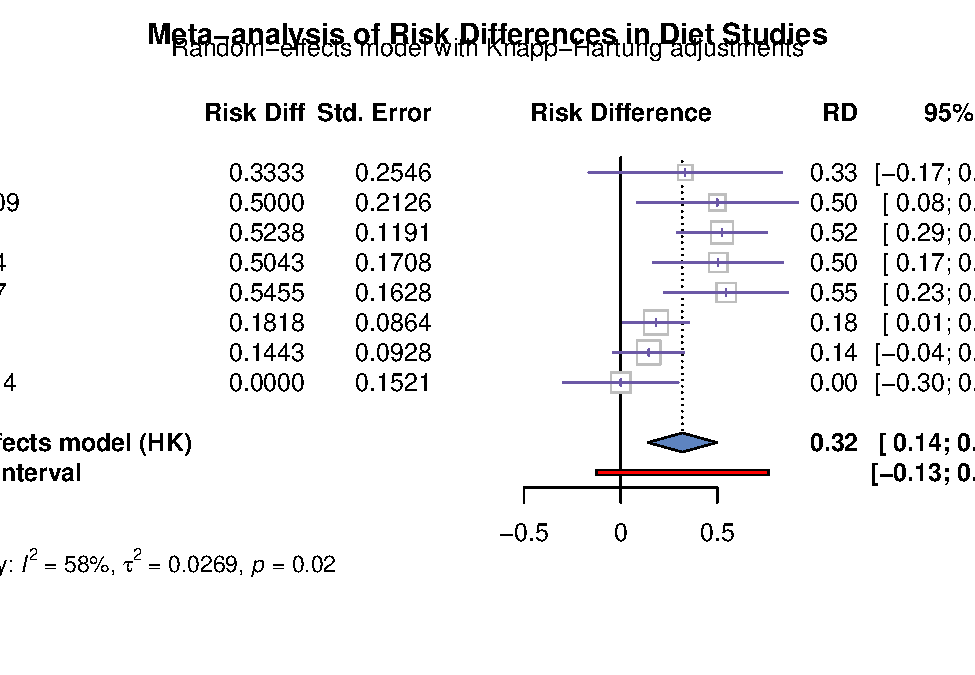
\includegraphics{_main_files/figure-latex/unnamed-chunk-30-1.pdf}

\subsection{Example 4: Orchard plots}\label{example-4-orchard-plots}

\begin{Shaded}
\begin{Highlighting}[]
\CommentTok{\# Load required libraries}
\FunctionTok{library}\NormalTok{(ggplot2)}
\FunctionTok{library}\NormalTok{(dplyr)}
\FunctionTok{library}\NormalTok{(metafor)}
\FunctionTok{library}\NormalTok{(ggbeeswarm)}

\CommentTok{\# Create a larger randomized dataset with valid constraints}
\FunctionTok{set.seed}\NormalTok{(}\DecValTok{42}\NormalTok{)  }\CommentTok{\# For reproducibility}
\NormalTok{n\_studies }\OtherTok{\textless{}{-}} \DecValTok{30}  \CommentTok{\# Total number of studies}

\NormalTok{dat }\OtherTok{\textless{}{-}} \FunctionTok{data.frame}\NormalTok{(}
  \AttributeTok{author =} \FunctionTok{paste}\NormalTok{(}\StringTok{"Study"}\NormalTok{, }\DecValTok{1}\SpecialCharTok{:}\NormalTok{n\_studies),}
  \AttributeTok{year =} \FunctionTok{sample}\NormalTok{(}\DecValTok{2000}\SpecialCharTok{:}\DecValTok{2020}\NormalTok{, n\_studies, }\AttributeTok{replace =} \ConstantTok{TRUE}\NormalTok{),}
  \AttributeTok{n1i =} \FunctionTok{sample}\NormalTok{(}\DecValTok{10}\SpecialCharTok{:}\DecValTok{100}\NormalTok{, n\_studies, }\AttributeTok{replace =} \ConstantTok{TRUE}\NormalTok{),  }\CommentTok{\# Total in experimental group}
  \AttributeTok{n2i =} \FunctionTok{sample}\NormalTok{(}\DecValTok{10}\SpecialCharTok{:}\DecValTok{100}\NormalTok{, n\_studies, }\AttributeTok{replace =} \ConstantTok{TRUE}\NormalTok{)   }\CommentTok{\# Total in control group}
\NormalTok{)}

\CommentTok{\# Randomly generate events ensuring that events do not exceed group sizes}
\NormalTok{dat}\SpecialCharTok{$}\NormalTok{ai }\OtherTok{\textless{}{-}} \FunctionTok{sapply}\NormalTok{(}\DecValTok{1}\SpecialCharTok{:}\NormalTok{n\_studies, }\ControlFlowTok{function}\NormalTok{(i) }\FunctionTok{sample}\NormalTok{(}\DecValTok{0}\SpecialCharTok{:}\NormalTok{dat}\SpecialCharTok{$}\NormalTok{n1i[i], }\DecValTok{1}\NormalTok{))  }\CommentTok{\# Events in experimental group}
\NormalTok{dat}\SpecialCharTok{$}\NormalTok{ci }\OtherTok{\textless{}{-}} \FunctionTok{sapply}\NormalTok{(}\DecValTok{1}\SpecialCharTok{:}\NormalTok{n\_studies, }\ControlFlowTok{function}\NormalTok{(i) }\FunctionTok{sample}\NormalTok{(}\DecValTok{0}\SpecialCharTok{:}\NormalTok{dat}\SpecialCharTok{$}\NormalTok{n2i[i], }\DecValTok{1}\NormalTok{))  }\CommentTok{\# Events in control group}

\CommentTok{\# Calculate risk differences}
\NormalTok{dat }\OtherTok{\textless{}{-}} \FunctionTok{escalc}\NormalTok{(}\AttributeTok{measure =} \StringTok{"RD"}\NormalTok{, }\AttributeTok{ai =}\NormalTok{ ai, }\AttributeTok{n1i =}\NormalTok{ n1i, }\AttributeTok{ci =}\NormalTok{ ci, }\AttributeTok{n2i =}\NormalTok{ n2i, }\AttributeTok{data =}\NormalTok{ dat)}

\CommentTok{\# Fit a random{-}effects model and create a subgroup variable}
\NormalTok{dat}\SpecialCharTok{$}\NormalTok{subgroup }\OtherTok{\textless{}{-}} \FunctionTok{sample}\NormalTok{(}\FunctionTok{c}\NormalTok{(}\StringTok{"Group A"}\NormalTok{, }\StringTok{"Group B"}\NormalTok{, }\StringTok{"Group C"}\NormalTok{), n\_studies, }\AttributeTok{replace =} \ConstantTok{TRUE}\NormalTok{)}

\CommentTok{\# Create an empty plot list to store individual subgroup plots}
\NormalTok{plot\_list }\OtherTok{\textless{}{-}} \FunctionTok{list}\NormalTok{()}

\CommentTok{\# Loop over each subgroup to create the overall mean for each}
\ControlFlowTok{for}\NormalTok{ (group }\ControlFlowTok{in} \FunctionTok{unique}\NormalTok{(dat}\SpecialCharTok{$}\NormalTok{subgroup)) \{}
\NormalTok{  subgroup\_data }\OtherTok{\textless{}{-}}\NormalTok{ dat[dat}\SpecialCharTok{$}\NormalTok{subgroup }\SpecialCharTok{==}\NormalTok{ group, ]}
\NormalTok{  res }\OtherTok{\textless{}{-}} \FunctionTok{rma}\NormalTok{(yi, vi, }\AttributeTok{data =}\NormalTok{ subgroup\_data, }\AttributeTok{method =} \StringTok{"DL"}\NormalTok{)  }\CommentTok{\# Fit model for subgroup}

  \CommentTok{\# Create the orchard plot for each subgroup}
\NormalTok{  p }\OtherTok{\textless{}{-}} \FunctionTok{ggplot}\NormalTok{(subgroup\_data, }\FunctionTok{aes}\NormalTok{(}\AttributeTok{x =}\NormalTok{ yi, }\AttributeTok{y =} \DecValTok{1}\NormalTok{)) }\SpecialCharTok{+}
    \FunctionTok{geom\_violin}\NormalTok{(}\AttributeTok{fill =} \StringTok{"lightgray"}\NormalTok{, }\AttributeTok{alpha =} \FloatTok{0.5}\NormalTok{) }\SpecialCharTok{+}
    \FunctionTok{geom\_quasirandom}\NormalTok{(}\FunctionTok{aes}\NormalTok{(}\AttributeTok{size =} \DecValTok{1}\SpecialCharTok{/}\FunctionTok{sqrt}\NormalTok{(vi)), }\AttributeTok{alpha =} \FloatTok{0.7}\NormalTok{) }\SpecialCharTok{+}  \CommentTok{\# Use inverse of SE for size}
    \FunctionTok{geom\_point}\NormalTok{(}\FunctionTok{aes}\NormalTok{(}\AttributeTok{x =}\NormalTok{ res}\SpecialCharTok{$}\NormalTok{b, }\AttributeTok{y =} \DecValTok{1}\NormalTok{, }\AttributeTok{color =} \StringTok{"Overall Mean"}\NormalTok{), }\AttributeTok{size =} \DecValTok{5}\NormalTok{, }\AttributeTok{shape =} \DecValTok{18}\NormalTok{) }\SpecialCharTok{+}
    \FunctionTok{geom\_errorbarh}\NormalTok{(}\FunctionTok{aes}\NormalTok{(}\AttributeTok{xmin =}\NormalTok{ res}\SpecialCharTok{$}\NormalTok{ci.lb, }\AttributeTok{xmax =}\NormalTok{ res}\SpecialCharTok{$}\NormalTok{ci.ub, }\AttributeTok{y =} \DecValTok{1}\NormalTok{), }\AttributeTok{height =} \FloatTok{0.1}\NormalTok{, }\AttributeTok{color =} \StringTok{"red"}\NormalTok{) }\SpecialCharTok{+}
    \FunctionTok{labs}\NormalTok{(}\AttributeTok{x =} \StringTok{"Risk Difference"}\NormalTok{, }\AttributeTok{y =} \StringTok{""}\NormalTok{, }\AttributeTok{title =} \FunctionTok{paste}\NormalTok{(}\StringTok{"Orchard Plot for"}\NormalTok{, group)) }\SpecialCharTok{+}
    \FunctionTok{scale\_color\_manual}\NormalTok{(}\AttributeTok{name =} \StringTok{""}\NormalTok{, }\AttributeTok{values =} \FunctionTok{c}\NormalTok{(}\StringTok{"Overall Mean"} \OtherTok{=} \StringTok{"red"}\NormalTok{)) }\SpecialCharTok{+}
    \FunctionTok{theme\_minimal}\NormalTok{() }\SpecialCharTok{+}
    \FunctionTok{theme}\NormalTok{(}\AttributeTok{axis.text.y =} \FunctionTok{element\_blank}\NormalTok{(), }\AttributeTok{axis.ticks.y =} \FunctionTok{element\_blank}\NormalTok{()) }\SpecialCharTok{+}
    \FunctionTok{xlim}\NormalTok{(}\FunctionTok{c}\NormalTok{(}\SpecialCharTok{{-}}\DecValTok{1}\NormalTok{, }\DecValTok{1}\NormalTok{)) }\SpecialCharTok{+}
    \FunctionTok{scale\_size}\NormalTok{(}\AttributeTok{range =} \FunctionTok{c}\NormalTok{(}\DecValTok{2}\NormalTok{, }\DecValTok{5}\NormalTok{), }\AttributeTok{name =} \StringTok{"Precision"}\NormalTok{) }

  \CommentTok{\# Store the plot in the list}
\NormalTok{  plot\_list[[group]] }\OtherTok{\textless{}{-}}\NormalTok{ p}
\NormalTok{\}}

\CommentTok{\# Display all orchard plots for each subgroup}
\FunctionTok{library}\NormalTok{(gridExtra)}
\FunctionTok{do.call}\NormalTok{(grid.arrange, }\FunctionTok{c}\NormalTok{(plot\_list, }\AttributeTok{ncol =} \DecValTok{1}\NormalTok{))  }\CommentTok{\# Arrange plots in a single column}
\end{Highlighting}
\end{Shaded}

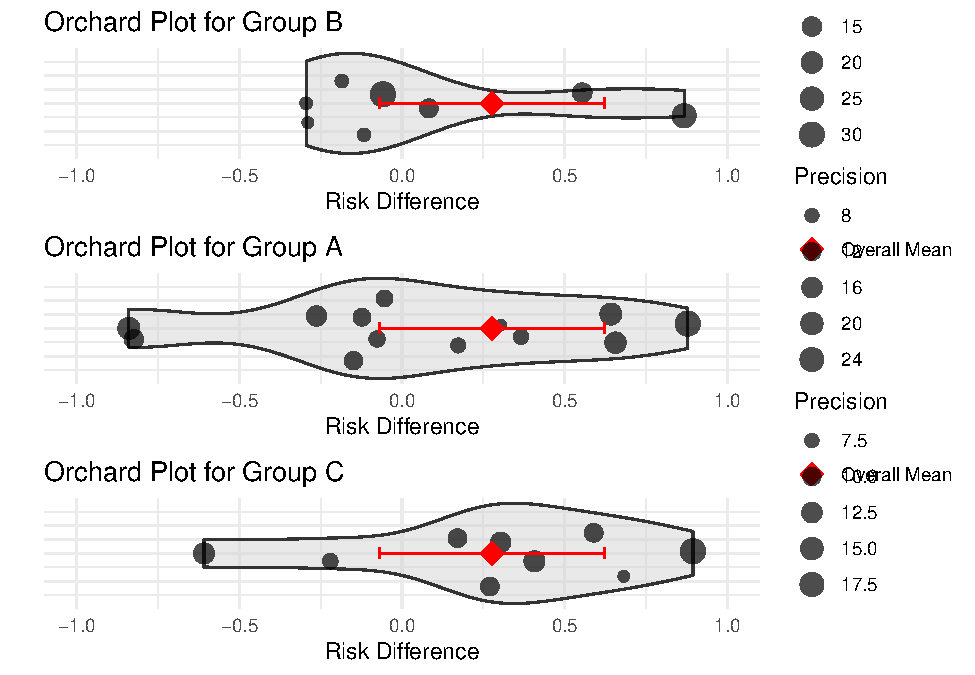
\includegraphics{_main_files/figure-latex/unnamed-chunk-31-1.pdf}

\chapter{Analysis and Visualization of Publication Bias}\label{analysis-and-visualization-of-publication-bias}

Publication bias is a significant concern in meta-analysis, as it can distort the overall effect estimate and lead to misleading conclusions. In this section, we will discuss various methods for detecting and visualizing publication bias, including funnel plots, the \emph{trim and fill} method, the Egger test, and Robust Bayesian Meta-Analysis.

\subsection{Funnel Plots}\label{funnel-plots}

A funnel plot is a scatter plot that helps visualize the relationship between the effect size and the precision of individual studies in a meta-analysis. It is an essential tool for identifying potential publication bias.

\begin{Shaded}
\begin{Highlighting}[]
\CommentTok{\# Load necessary libraries}
\FunctionTok{library}\NormalTok{(metafor)}
\FunctionTok{library}\NormalTok{(ggplot2)}

\CommentTok{\# Create a data frame with example data}
\NormalTok{data }\OtherTok{\textless{}{-}} \FunctionTok{data.frame}\NormalTok{(}
  \AttributeTok{study =} \FunctionTok{c}\NormalTok{(}\StringTok{"Study1"}\NormalTok{, }\StringTok{"Study2"}\NormalTok{, }\StringTok{"Study3"}\NormalTok{, }\StringTok{"Study4"}\NormalTok{, }\StringTok{"Study5"}\NormalTok{),}
  \AttributeTok{smd =} \FunctionTok{c}\NormalTok{(}\FloatTok{0.5}\NormalTok{, }\FloatTok{0.8}\NormalTok{, }\FloatTok{0.3}\NormalTok{, }\FloatTok{1.0}\NormalTok{, }\FloatTok{0.9}\NormalTok{),}
  \AttributeTok{var\_smd =} \FunctionTok{c}\NormalTok{(}\FloatTok{0.1}\NormalTok{, }\FloatTok{0.15}\NormalTok{, }\FloatTok{0.2}\NormalTok{, }\FloatTok{0.05}\NormalTok{, }\FloatTok{0.12}\NormalTok{)}
\NormalTok{)}

\CommentTok{\# Conduct a random{-}effects meta{-}analysis}
\NormalTok{res }\OtherTok{\textless{}{-}} \FunctionTok{rma}\NormalTok{(}\AttributeTok{yi =}\NormalTok{ smd, }\AttributeTok{vi =}\NormalTok{ var\_smd, }\AttributeTok{data =}\NormalTok{ data)}

\NormalTok{estimate }\OtherTok{\textless{}{-}}\NormalTok{ res}\SpecialCharTok{$}\NormalTok{b  }\CommentTok{\# Replace with your meta{-}analytic estimate if needed}
\NormalTok{se }\OtherTok{\textless{}{-}}\NormalTok{ res}\SpecialCharTok{$}\NormalTok{se        }\CommentTok{\# Replace with your standard error if needed}

\CommentTok{\# Define a sequence for standard errors (SE) to create CI regions}
\NormalTok{se.seq }\OtherTok{\textless{}{-}} \FunctionTok{seq}\NormalTok{(}\DecValTok{0}\NormalTok{, }\FunctionTok{max}\NormalTok{(data}\SpecialCharTok{$}\NormalTok{var\_smd), }\FloatTok{0.001}\NormalTok{)}

\CommentTok{\# Calculate 95\% and 99\% confidence intervals for the region}
\NormalTok{ll95 }\OtherTok{\textless{}{-}}\NormalTok{ estimate }\SpecialCharTok{{-}}\NormalTok{ (}\FloatTok{1.96} \SpecialCharTok{*}\NormalTok{ se.seq)}
\NormalTok{ul95 }\OtherTok{\textless{}{-}}\NormalTok{ estimate }\SpecialCharTok{+}\NormalTok{ (}\FloatTok{1.96} \SpecialCharTok{*}\NormalTok{ se.seq)}
\NormalTok{ll99 }\OtherTok{\textless{}{-}}\NormalTok{ estimate }\SpecialCharTok{{-}}\NormalTok{ (}\FloatTok{3.29} \SpecialCharTok{*}\NormalTok{ se.seq)}
\NormalTok{ul99 }\OtherTok{\textless{}{-}}\NormalTok{ estimate }\SpecialCharTok{+}\NormalTok{ (}\FloatTok{3.29} \SpecialCharTok{*}\NormalTok{ se.seq)}

\CommentTok{\# Compute confidence intervals for the mean meta{-}analytic estimate}
\NormalTok{meanll95 }\OtherTok{\textless{}{-}}\NormalTok{ estimate }\SpecialCharTok{{-}}\NormalTok{ (}\FloatTok{1.96} \SpecialCharTok{*}\NormalTok{ se)}
\NormalTok{meanul95 }\OtherTok{\textless{}{-}}\NormalTok{ estimate }\SpecialCharTok{+}\NormalTok{ (}\FloatTok{1.96} \SpecialCharTok{*}\NormalTok{ se)}

\CommentTok{\# Store all calculated values in a single data frame for easy plotting}
\NormalTok{dfCI }\OtherTok{\textless{}{-}} \FunctionTok{data.frame}\NormalTok{(ll95, ul95, ll99, ul99, se.seq, estimate, meanll95, meanul95)}


\CommentTok{\# Draw the enhanced funnel plot with shaded CI regions and lines}
\NormalTok{funnel\_plot }\OtherTok{\textless{}{-}} \FunctionTok{ggplot}\NormalTok{(}\FunctionTok{aes}\NormalTok{(}\AttributeTok{x =}\NormalTok{ var\_smd, }\AttributeTok{y =}\NormalTok{ smd), }\AttributeTok{data =}\NormalTok{ data)}\SpecialCharTok{+}
  \CommentTok{\# Add shaded areas for 95\% and 99\% CI regions}
  \FunctionTok{geom\_point}\NormalTok{(}\AttributeTok{shape =} \DecValTok{1}\NormalTok{) }\SpecialCharTok{+}
  \FunctionTok{xlab}\NormalTok{(}\StringTok{\textquotesingle{}Standard Error\textquotesingle{}}\NormalTok{) }\SpecialCharTok{+} \FunctionTok{ylab}\NormalTok{(}\StringTok{\textquotesingle{}smd\textquotesingle{}}\NormalTok{)}\SpecialCharTok{+}
  \FunctionTok{geom\_line}\NormalTok{(}\FunctionTok{aes}\NormalTok{(}\AttributeTok{x =}\NormalTok{ se.seq, }\AttributeTok{y =}\NormalTok{ ll95), }\AttributeTok{linetype =} \StringTok{\textquotesingle{}dotted\textquotesingle{}}\NormalTok{, }\AttributeTok{data =}\NormalTok{ dfCI) }\SpecialCharTok{+}
  \FunctionTok{geom\_line}\NormalTok{(}\FunctionTok{aes}\NormalTok{(}\AttributeTok{x =}\NormalTok{ se.seq, }\AttributeTok{y =}\NormalTok{ ul95), }\AttributeTok{linetype =} \StringTok{\textquotesingle{}dotted\textquotesingle{}}\NormalTok{, }\AttributeTok{data =}\NormalTok{ dfCI) }\SpecialCharTok{+}
  \FunctionTok{geom\_line}\NormalTok{(}\FunctionTok{aes}\NormalTok{(}\AttributeTok{x =}\NormalTok{ se.seq, }\AttributeTok{y =}\NormalTok{ ll99), }\AttributeTok{linetype =} \StringTok{\textquotesingle{}dashed\textquotesingle{}}\NormalTok{, }\AttributeTok{data =}\NormalTok{ dfCI) }\SpecialCharTok{+}
  \FunctionTok{geom\_line}\NormalTok{(}\FunctionTok{aes}\NormalTok{(}\AttributeTok{x =}\NormalTok{ se.seq, }\AttributeTok{y =}\NormalTok{ ul99), }\AttributeTok{linetype =} \StringTok{\textquotesingle{}dashed\textquotesingle{}}\NormalTok{, }\AttributeTok{data =}\NormalTok{ dfCI) }\SpecialCharTok{+}
  \FunctionTok{geom\_segment}\NormalTok{(}\FunctionTok{aes}\NormalTok{(}\AttributeTok{x =} \FunctionTok{min}\NormalTok{(se.seq), }\AttributeTok{y =}\NormalTok{ meanll95, }\AttributeTok{xend =} \FunctionTok{max}\NormalTok{(se.seq), }\AttributeTok{yend =}\NormalTok{ meanll95), }\AttributeTok{linetype=}\StringTok{\textquotesingle{}dotted\textquotesingle{}}\NormalTok{, }\AttributeTok{data=}\NormalTok{dfCI) }\SpecialCharTok{+}
  \FunctionTok{geom\_segment}\NormalTok{(}\FunctionTok{aes}\NormalTok{(}\AttributeTok{x =} \FunctionTok{min}\NormalTok{(se.seq), }\AttributeTok{y =}\NormalTok{ meanul95, }\AttributeTok{xend =} \FunctionTok{max}\NormalTok{(se.seq), }\AttributeTok{yend =}\NormalTok{ meanul95), }\AttributeTok{linetype=}\StringTok{\textquotesingle{}dotted\textquotesingle{}}\NormalTok{, }\AttributeTok{data=}\NormalTok{dfCI) }\SpecialCharTok{+}
  \FunctionTok{scale\_x\_reverse}\NormalTok{()}\SpecialCharTok{+}
  \FunctionTok{scale\_y\_continuous}\NormalTok{(}\AttributeTok{breaks=}\FunctionTok{seq}\NormalTok{(}\SpecialCharTok{{-}}\FloatTok{1.25}\NormalTok{,}\DecValTok{2}\NormalTok{,}\FloatTok{0.25}\NormalTok{))}\SpecialCharTok{+}
  \FunctionTok{coord\_flip}\NormalTok{()}\SpecialCharTok{+}
  \FunctionTok{theme\_bw}\NormalTok{()}

\CommentTok{\# Display the enhanced funnel plot}
\NormalTok{funnel\_plot}
\end{Highlighting}
\end{Shaded}

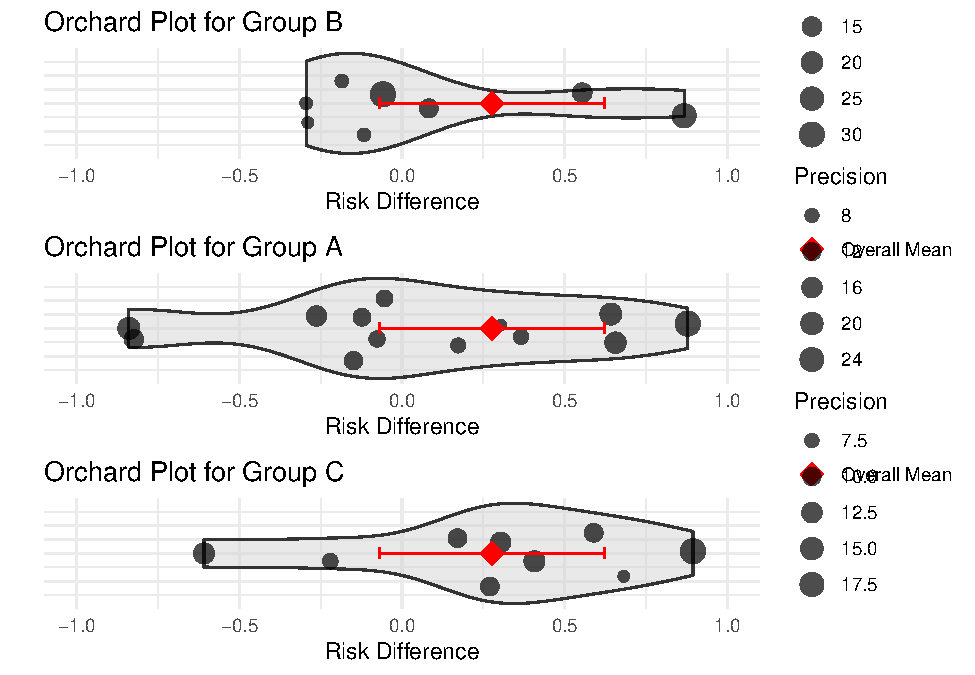
\includegraphics{_main_files/figure-latex/unnamed-chunk-32-1.pdf}

\subsubsection{Understanding Funnel Plots}\label{understanding-funnel-plots}

\begin{itemize}
\item
  \textbf{Structure}: In an ideal scenario, a funnel plot resembles an inverted funnel or a pyramid. This shape reflects that larger studies tend to be more precise (higher up on the plot), while smaller studies have more variability (scattered at the bottom).
\item
  \textbf{Axes}:

  \begin{itemize}
  \item
    The \textbf{x-axis} represents the estimated effect size for each study (e.g., risk ratios, odds ratios plotted on a logarithmic scale, or mean differences).
  \item
    The \textbf{y-axis} indicates the study precision, often measured by the standard error. Larger studies with greater precision are displayed at the top.
  \end{itemize}
\end{itemize}

In a bias-free scenario, 95\% of studies would be expected to lie within the dashed lines representing the 95\% confidence interval.

\subsubsection{Interpreting Funnel Plots}\label{interpreting-funnel-plots}

When analyzing a funnel plot, look for symmetry. A symmetrical plot suggests that publication bias is unlikely, while an asymmetrical plot may indicate bias. \textbf{Image B} illustrates an asymmetrical funnel, where points predominantly cluster on one side, suggesting that the summary estimate may overstate the effect.

\subsection{Reasons for Asymmetry}\label{reasons-for-asymmetry}

Asymmetry in a funnel plot can arise from several factors:

\begin{itemize}
\item
  \textbf{Non-reporting Bias}: Studies with non-significant results may be less likely to be published.
\item
  \textbf{Methodological Quality}: Studies with poor design may report exaggerated effect sizes.
\item
  \textbf{True Heterogeneity}: Variability in patient populations can lead to biased estimates, especially in smaller studies.
\item
  \textbf{Artefactual Correlation}: Correlations between effect estimates and their standard errors can create false asymmetry.
\item
  \textbf{Chance}: Random variation is more likely in analyses with fewer studies.
\end{itemize}

\subsection{Trim and Fill Method}\label{trim-and-fill-method}

The \emph{trim and fill} method adjusts for publication bias by estimating the number of studies that would need to be added to achieve symmetry. This method imputes missing studies to provide a more accurate effect size.

\subsubsection{Example of Using Trim and Fill}\label{example-of-using-trim-and-fill}

\begin{Shaded}
\begin{Highlighting}[]
\CommentTok{\# Perform trim and fill analysis}
\NormalTok{trimmed\_res }\OtherTok{\textless{}{-}} \FunctionTok{trimfill}\NormalTok{(res)}

\CommentTok{\# Summary of the results}
\FunctionTok{summary}\NormalTok{(trimmed\_res)}
\end{Highlighting}
\end{Shaded}

\begin{verbatim}
## 
## Estimated number of missing studies on the right side: 1 (SE = 1.7009)
## 
## Random-Effects Model (k = 6; tau^2 estimator: REML)
## 
##   logLik  deviance       AIC       BIC      AICc   
##  -1.7515    3.5031    7.5031    6.7219   13.5031   
## 
## tau^2 (estimated amount of total heterogeneity): 0.0000 (SE = 0.0673)
## tau (square root of estimated tau^2 value):      0.0022
## I^2 (total heterogeneity / total variability):   0.00%
## H^2 (total variability / sampling variability):  1.00
## 
## Test for Heterogeneity:
## Q(df = 5) = 4.6326, p-val = 0.4623
## 
## Model Results:
## 
## estimate      se    zval    pval   ci.lb   ci.ub      
##   0.8407  0.1348  6.2349  <.0001  0.5764  1.1050  *** 
## 
## ---
## Signif. codes:  0 '***' 0.001 '**' 0.01 '*' 0.05 '.' 0.1 ' ' 1
\end{verbatim}

\begin{Shaded}
\begin{Highlighting}[]
\CommentTok{\# Create a funnel plot with imputed studies}
\FunctionTok{funnel}\NormalTok{(trimmed\_res, }\AttributeTok{main =} \StringTok{"Funnel Plot with Trim and Fill"}\NormalTok{)}
\end{Highlighting}
\end{Shaded}

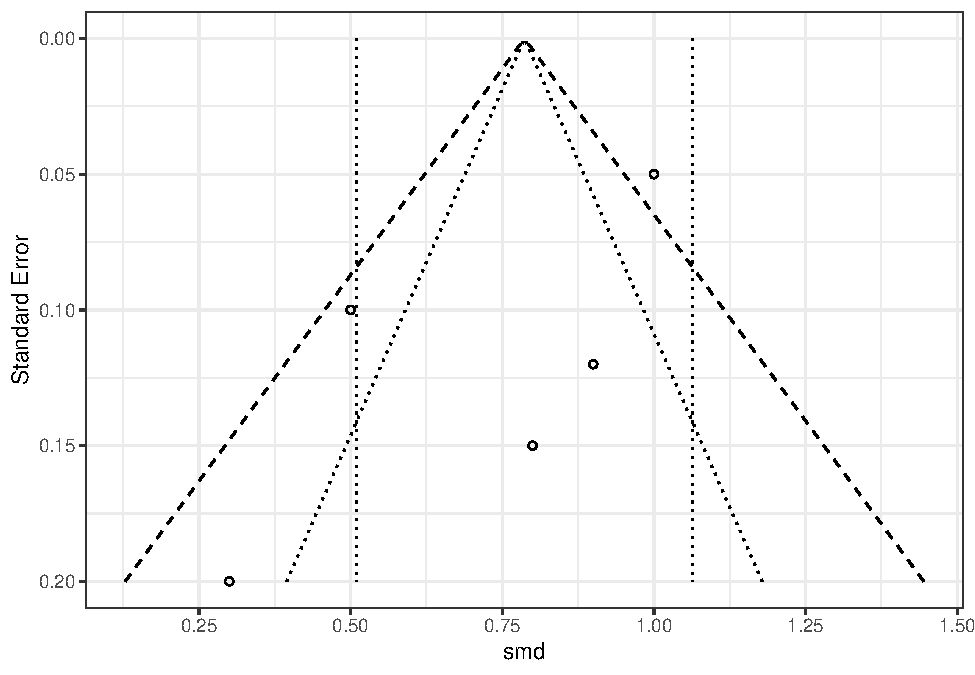
\includegraphics{_main_files/figure-latex/unnamed-chunk-33-1.pdf}

In this example, the \texttt{trimfill} function from the \texttt{metafor} package adjusts the meta-analysis results for publication bias.

\subsection{Duval and Tweedie's Trim and Fill}\label{duval-and-tweedies-trim-and-fill}

An alternative to the traditional \emph{trim and fill}, Duval and Tweedie's method provides an updated approach to adjust for publication bias, offering more robust imputation of missing studies.

\subsubsection{Example of Using Duval and Tweedie's Method}\label{example-of-using-duval-and-tweedies-method}

\begin{Shaded}
\begin{Highlighting}[]
\CommentTok{\# Perform Duval and Tweedie\textquotesingle{}s trim and fill}
\NormalTok{duval\_tweedie\_res }\OtherTok{\textless{}{-}} \FunctionTok{trimfill}\NormalTok{(res, }\AttributeTok{direction =} \StringTok{"both"}\NormalTok{)}

\CommentTok{\# Create a funnel plot with Duval and Tweedie’s imputation}
\FunctionTok{funnel}\NormalTok{(duval\_tweedie\_res, }\AttributeTok{main =} \StringTok{"Funnel Plot with Duval and Tweedie\textquotesingle{}s Trim and Fill"}\NormalTok{)}
\end{Highlighting}
\end{Shaded}

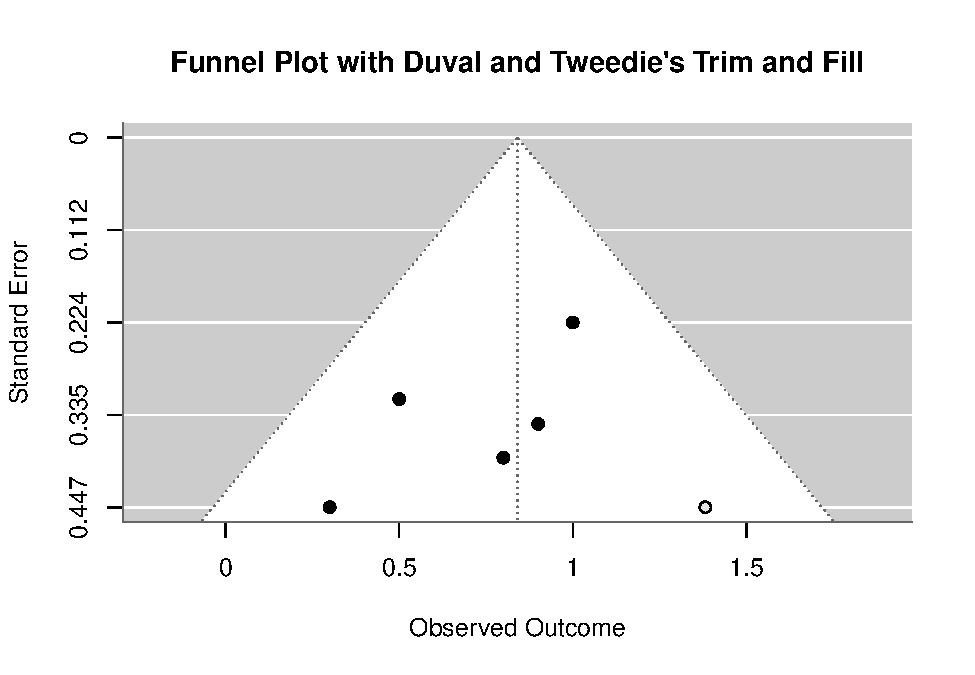
\includegraphics{_main_files/figure-latex/unnamed-chunk-34-1.pdf}

\subsection{3. Egger Test}\label{egger-test}

The Egger test statistically assesses funnel plot asymmetry. A significant result indicates potential publication bias.

\subsubsection{Conducting the Egger Test}\label{conducting-the-egger-test}

\begin{Shaded}
\begin{Highlighting}[]
\CommentTok{\# Conduct the Egger test}
\NormalTok{egger\_test }\OtherTok{\textless{}{-}} \FunctionTok{regtest}\NormalTok{(res)}

\CommentTok{\# Display the test results}
\FunctionTok{print}\NormalTok{(egger\_test)}
\end{Highlighting}
\end{Shaded}

\begin{verbatim}
## 
## Regression Test for Funnel Plot Asymmetry
## 
## Model:     mixed-effects meta-regression model
## Predictor: standard error
## 
## Test for Funnel Plot Asymmetry: z = -1.2521, p = 0.2105
## Limit Estimate (as sei -> 0):   b =  1.4949 (CI: 0.3521, 2.6376)
\end{verbatim}

\subsection{Rosenthal's Fail-Safe N}\label{rosenthals-fail-safe-n}

Rosenthal's Fail-Safe N calculates the number of unpublished studies with null results needed to invalidate the overall effect. A high Fail-Safe N suggests that publication bias is unlikely to significantly impact the findings.

\subsubsection{Example of Calculating Fail-Safe N}\label{example-of-calculating-fail-safe-n}

\begin{Shaded}
\begin{Highlighting}[]
\CommentTok{\# Calculate the Fail{-}Safe N}
\NormalTok{failsafe\_n }\OtherTok{\textless{}{-}} \FunctionTok{fsn}\NormalTok{(res)}
\FunctionTok{print}\NormalTok{(failsafe\_n)}
\end{Highlighting}
\end{Shaded}

\begin{verbatim}
## 
## Fail-safe N Calculation Using the General Approach
## 
## Average Effect Size:         0.7867 (with file drawer: 0.2950)
## Amount of Heterogeneity:     0.0000 (with file drawer: 0.1641)
## Observed Significance Level: <.0001 (with file drawer: 0.0493)
## Target Significance Level:   0.05
## 
## Fail-safe N: 8
\end{verbatim}

\subsubsection{Robust Bayesian Meta-Analysis (RoBMA)}\label{robust-bayesian-meta-analysis-robma}

\textbf{Robust Bayesian Meta-Analysis (RoBMA)} is an advanced method designed to address the limitations of traditional meta-analysis by incorporating information on publication bias, heterogeneity, and effect sizes in a single model. It relies on Bayesian principles to estimate the probability of the presence of a real effect while considering the potential for biases and study variability. RoBMA extends the traditional meta-analytic framework by integrating multiple models that account for different sources of uncertainty. It not only provides point estimates of effect sizes but also outputs the probability that publication bias and heterogeneity are influencing the results. This allows for a more transparent and reliable evaluation of the evidence base. Specifically, RoBMA offers:

\begin{itemize}
\item
  \textbf{Probabilistic conclusions}: Instead of simple yes/no results, RoBMA provides probabilities for the presence of effects, heterogeneity, and bias.
\item
  \textbf{Robust model averaging}: It combines estimates across different models, reducing sensitivity to outliers and small study effects.
\item
  \textbf{Enhanced diagnostics}: RoBMA provides visual tools to detect and correct for bias, making it easier to understand and communicate findings.
\end{itemize}

\subsubsection{Setting Up and Running a RoBMA Model in R}\label{setting-up-and-running-a-robma-model-in-r}

The implementation of RoBMA in R is straightforward using the \texttt{RoBMA} package. Below is a basic example using simulated effect sizes (\texttt{d}) and standard errors (\texttt{se}):

\begin{Shaded}
\begin{Highlighting}[]
\CommentTok{\# Load the necessary libraries}
\FunctionTok{library}\NormalTok{(RoBMA)}
\end{Highlighting}
\end{Shaded}

\begin{verbatim}
## Loading required namespace: runjags
\end{verbatim}

\begin{verbatim}
## 
## Attaching package: 'RoBMA'
\end{verbatim}

\begin{verbatim}
## The following object is masked from 'package:brms':
## 
##     prior
\end{verbatim}

\begin{verbatim}
## The following object is masked from 'package:meta':
## 
##     forest
\end{verbatim}

\begin{verbatim}
## The following object is masked from 'package:metafor':
## 
##     forest
\end{verbatim}

\begin{Shaded}
\begin{Highlighting}[]
\CommentTok{\# Ensure your dataset \textquotesingle{}dat\textquotesingle{} is structured correctly}
\CommentTok{\# Use the yi and vi columns from \textquotesingle{}dat\textquotesingle{}}
\CommentTok{\# Fit the Bayesian meta{-}analysis model}
\NormalTok{fit }\OtherTok{\textless{}{-}} \FunctionTok{RoBMA}\NormalTok{(}
  \AttributeTok{d =}\NormalTok{ dat}\SpecialCharTok{$}\NormalTok{yi,                     }\CommentTok{\# Effect sizes}
  \AttributeTok{se =} \FunctionTok{sqrt}\NormalTok{(dat}\SpecialCharTok{$}\NormalTok{vi),              }\CommentTok{\# Standard errors from variances}
  \AttributeTok{study\_names =} \FunctionTok{as.character}\NormalTok{(dat}\SpecialCharTok{$}\NormalTok{paper),        }\CommentTok{\# Unique study identifiers}
  \AttributeTok{seed =} \DecValTok{1}\NormalTok{,                        }\CommentTok{\# Seed for reproducibility}
  \AttributeTok{chains =} \DecValTok{2}\NormalTok{,}
  \AttributeTok{sample =} \DecValTok{500}\NormalTok{,}
  \AttributeTok{burnin =} \DecValTok{200}\NormalTok{,}\AttributeTok{parallel =} \ConstantTok{TRUE}\NormalTok{)}

\CommentTok{\# Summarize the results}
\FunctionTok{summary}\NormalTok{(fit)}
\end{Highlighting}
\end{Shaded}

\begin{verbatim}
## Call:
## RoBMA(d = dat$yi, se = sqrt(dat$vi), study_names = as.character(dat$paper), 
##     chains = 2, sample = 500, burnin = 200, parallel = TRUE, 
##     seed = 1)
## 
## Robust Bayesian meta-analysis
## Components summary:
##               Models Prior prob. Post. prob. Inclusion BF
## Effect         18/36       0.500       0.171        0.206
## Heterogeneity  18/36       0.500       1.000          Inf
## Bias           32/36       0.500       0.359        0.560
## 
## Model-averaged estimates:
##                    Mean Median 0.025 0.975
## mu                0.018  0.000 0.000 0.204
## tau               0.479  0.472 0.373 0.628
## omega[0,0.025]    1.000  1.000 1.000 1.000
## omega[0.025,0.05] 0.992  1.000 0.873 1.000
## omega[0.05,0.5]   0.969  1.000 0.572 1.000
## omega[0.5,0.95]   0.965  1.000 0.529 1.000
## omega[0.95,0.975] 0.967  1.000 0.541 1.000
## omega[0.975,1]    0.969  1.000 0.541 1.000
## PET               0.099  0.000 0.000 1.183
## PEESE             0.500  0.000 0.000 6.212
## The estimates are summarized on the Cohen's d scale (priors were specified on the Cohen's d scale).
## (Estimated publication weights omega correspond to one-sided p-values.)
\end{verbatim}

\begin{Shaded}
\begin{Highlighting}[]
\CommentTok{\# Plot the results for the parameter of interest}
\FunctionTok{plot}\NormalTok{(fit, }\AttributeTok{parameter =} \StringTok{"mu"}\NormalTok{, }\AttributeTok{xlim =} \FunctionTok{c}\NormalTok{(}\SpecialCharTok{{-}}\FloatTok{0.5}\NormalTok{, }\FloatTok{0.5}\NormalTok{))  }\CommentTok{\# Adjust xlim as necessary}
\end{Highlighting}
\end{Shaded}

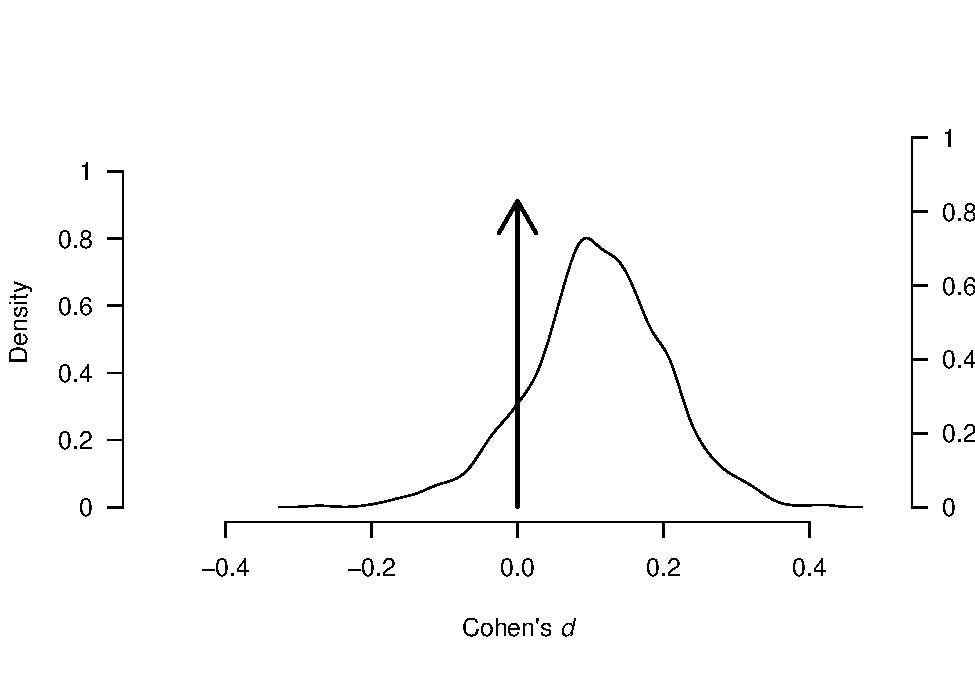
\includegraphics{_main_files/figure-latex/unnamed-chunk-37-1.pdf}

\subsubsection{Key Outputs and Interpretation}\label{key-outputs-and-interpretation}

\begin{enumerate}
\def\labelenumi{\arabic{enumi}.}
\item
  \textbf{Model Components and Inclusion Probabilities}:

  RoBMA assesses three primary components: Effect, Heterogeneity, and Bias. The \emph{Inclusion Probability} indicates how likely each component is part of the model:

  \begin{itemize}
  \item
    \textbf{Effect}: Probability that a true non-zero effect exists.
  \item
    \textbf{Heterogeneity}: Probability that effect sizes vary significantly between studies.
  \item
    \textbf{Bias}: Probability that results are influenced by publication bias.
  \end{itemize}

  For example, if \texttt{Bias\ =\ 98\%}, this suggests a very high likelihood that publication bias is present and impacting the results.
\item
  \textbf{Model-Averaged Estimates}:

  RoBMA reports \emph{model-averaged} estimates for the average effect size (\texttt{mu}), between-study variance (\texttt{tau}), and other model parameters. This averaging reduces the impact of individual extreme results by incorporating information from all candidate models.

  \begin{itemize}
  \item
    \texttt{mu}: The central tendency of the effect size (e.g., Cohen's \emph{d}).
  \item
    \texttt{tau}: The estimated heterogeneity, reflecting how much the effect sizes vary between studies.
  \item
    \textbf{Bias Weights (\texttt{omega})}: These weights correspond to the probability of study inclusion based on their p-values, directly indicating the severity of publication bias.
  \end{itemize}
\item
  \textbf{Posterior Model Probabilities}:

  Each model in RoBMA has a posterior probability, which tells you how well that specific combination of effect, heterogeneity, and bias explains the observed data. This helps in identifying the most plausible scenarios.
\end{enumerate}

\subsubsection{Visualizing Publication Bias with RoBMA}\label{visualizing-publication-bias-with-robma}

RoBMA provides tools to visually inspect and diagnose publication bias using enhanced funnel plots. To generate a funnel plot that shows bias-corrected effects, you can use:

\begin{Shaded}
\begin{Highlighting}[]
\CommentTok{\# Create an enhanced funnel plot with bias adjustment}
\FunctionTok{plot}\NormalTok{(fit, }\AttributeTok{type =} \StringTok{"funnel"}\NormalTok{, }\AttributeTok{show\_legend =} \ConstantTok{TRUE}\NormalTok{)}
\end{Highlighting}
\end{Shaded}

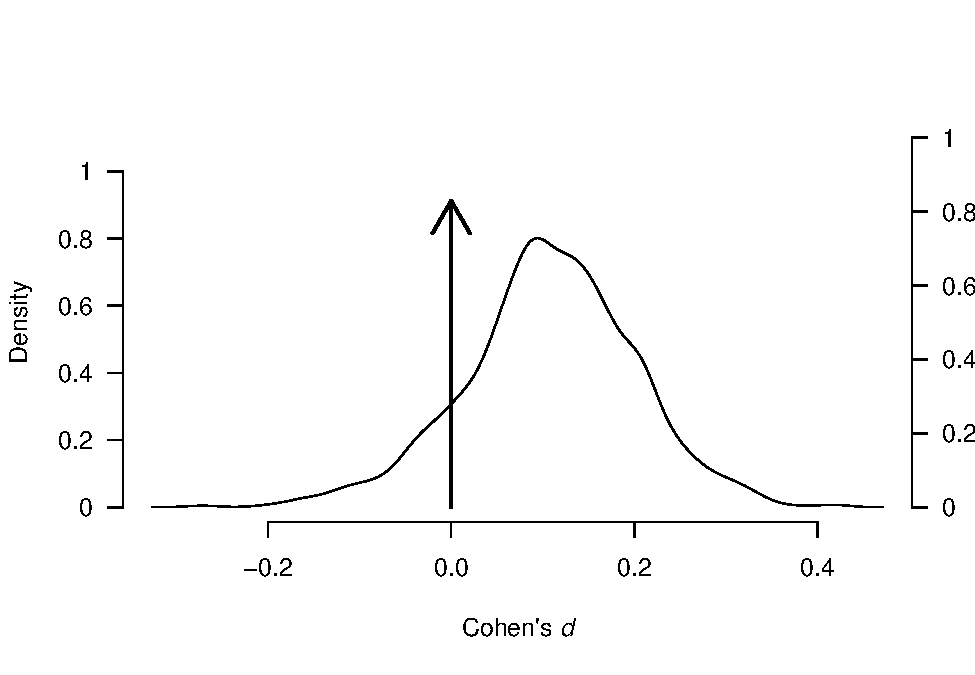
\includegraphics{_main_files/figure-latex/unnamed-chunk-38-1.pdf}

The enhanced funnel plot compares the original effect sizes with those adjusted for potential biases. Asymmetry or clustering patterns in the plot indicate possible biases, while the adjusted estimates provide a more accurate picture of the underlying effect.

\subsubsection{Advantages of Using RoBMA}\label{advantages-of-using-robma}

\begin{itemize}
\item
  \textbf{Comprehensive Bias Assessment}: RoBMA integrates several models to check for the presence and impact of publication bias.
\item
  \textbf{Flexible Prior Specification}: Allows for the use of both informative and non-informative priors, adapting to various research scenarios.
\item
  \textbf{Model-Averaging for Stability}: By combining different models, RoBMA reduces the chance of overfitting and provides more robust conclusions.
\end{itemize}

\subsubsection{Limitations to Consider}\label{limitations-to-consider}

\begin{itemize}
\item
  \textbf{Computational Complexity}: Running RoBMA with large datasets or complex prior structures can be resource-intensive.
\item
  \textbf{Advanced Interpretation}: Understanding and explaining RoBMA results may require familiarity with Bayesian concepts and model averaging.
\end{itemize}

  \bibliography{book.bib,packages.bib}

\end{document}
